\documentclass{article}
\usepackage[utf8]{inputenc}
\usepackage{amssymb}       % Librerías matemáticas
\usepackage{amsthm}        % Definición de teoremas
\usepackage{array}         % Nuevas características a las tablas
\usepackage{bigstrut}      % Líneas horizontales en tablas
\usepackage{bm}            % Caracteres en negrita en ecuaciones
\usepackage{booktabs}      % Permite manejar elementos visuales en tablas
\usepackage{caption}       % Leyendas
\usepackage{changepage}    % Condicionales para administrar páginas
\usepackage{chngcntr}      % Añade números a las leyendas
\usepackage{color}         % Colores
\usepackage{datetime}      % Fechas
\usepackage{enumitem}      % Listas con letras
\usepackage{floatpag}      % Maneja números de páginas
\usepackage{floatrow}      % Permite administrar posiciones en los caption
\usepackage{framed}        % Permite creación de recuadros
\usepackage{gensymb}       % Simbología común
\usepackage{graphicx}      % Propiedades extra para los gráficos
\usepackage{lipsum}        % Permite crear párrafos de prueba
\usepackage{listings}      % Permite añadir código fuente
\usepackage{longtable}     % Permite utilizar tablas en varias hojas
\usepackage{mathtools}     % Permite utilizar notaciones matemáticas
\usepackage{multicol}      % Múltiples columnas
\usepackage{needspace}     % Maneja los espacios en página
\usepackage{pdflscape}     % Modo página horizontal de página
\usepackage{pdfpages}      % Permite administrar páginas en pdf
\usepackage{physics}       % Paquete de matemáticas
% \usepackage{ragged2e}    % Redefine centering
\usepackage{rotating}      % Permite rotación de objetos
\usepackage{selinput}      % Compatibilidad con acentos
\usepackage{setspace}      % Cambia el espacio entre líneas
\usepackage{soul}          % Permite subrayar texto
\usepackage{subfig}        % Permite agrupar imágenes
\usepackage{textcomp}      % Simbología común
\usepackage{url}           % Permite añadir enlaces
\usepackage{wrapfig}       % Posición de imágenes
\usepackage{xspace}        % Adminsitra espacios en párrafos y líneas
\usepackage{amsmath}
%\usepackage{tikz}
\usepackage{mathdots}
\usepackage{yhmath}
\usepackage{cancel}
\usepackage{siunitx}
\usepackage{multirow}
\usepackage{tabularx}
\usepackage{xstring}
\usepackage[spanish,british]{babel}
\usepackage{hyperref}
\hypersetup{
    colorlinks=true,
    linkcolor=blue,
    filecolor=cyan,      
    urlcolor=magenta
}
\usepackage{titlesec}
%\usetikzlibrary{fadings}
%\usetikzlibrary{patterns}
%\usetikzlibrary{shadows.blur}
%\usetikzlibrary{shapes}


% ---- CONFIG ----

\titleformat{\section}
  {\Large\bfseries}{Módulo \thesection:}{10px}{}
 
\setcounter{section}{-1}

\newcommand{\econ}[2]{\textit{Capítulo correspondiente en CORE ECON: \href{#1}{Capítulo #2}}}

\newcommand{\fuente}[1]{\textit{[Fuente: #1]}}

\newcounter{problemas}[section]
\newcommand{\newpbm}{\stepcounter{problemas}\begin{flushleft}\boxed{\textbf{P.\thesection.\arabic{problemas}}} \hyperlink{S.\thesection.\arabic{problemas}}{Sol} \end{flushleft}
\hfill\\}  % Permite crear problema con ajuste de número y sección automático

\newcommand{\np}{\newpbm} % Alias por si prefieres

\newenvironment{solucion}[1]{
    \hfill\\
    \hypertarget{S.\thesection.#1}
    \text{}\boxed{\textbf{S.\thesection.#1}}
    \hfill\\
    }{}

% Cita o comillas " "
% Modo de uso: \cita{ texto }
\newcommand{\cita}[1]{``#1''}

% Superíndice text
% Modo de uso: \txtsi{ texto }{ objeto que irá en el índice }
\newcommand{\txtsi}[2]{$\text{#1}^{#2}$}

% Paréntesis grandes en comando 
% Modo de uso: \lados{ tipo de parentésis }{ Ecuación }
% Requisitos: \usepackage{xstring}
\newcommand{\lados}[2]{%
    \IfEqCase{#1}{%
        {(}{\left( #2 \right)}%
        {)}{\left( #2 \right)}%
        {()}{\left( #2 \right)}%
        {[}{\left[ #2 \right]}%
        {]}{\left[ #2 \right]}%
        {[]}{\left[ #2 \right]}%
        {\{}{\left\{ #2 \right\}}%
        {\}}{\left\{ #2 \right\}}%
        {\lfloor}{\left\lfloor #2 \right\rfloor}%
        {\rfloor}{\left\lfloor #2 \right\rfloor}%
    }[\PackageError{lados}{Opción no definida: #1}{}]%
}%

% ---- END CONFIG ----

\title{Economía IN2201}
\author{\textit{Le Touffe}}
\date{\monthname\text{ 2020}}


\begin{document}

\maketitle
\begin{abstract}
    \begin{center}
        
    
	Información pertinente al ramo de economía del 
	
	semestre primavera 2020. 
	
	Se recomienda vehemente leer el CORE en los módulos donde es posible, esto es un simple 'apunte'.
	\end{center}
\end{abstract}
\selectlanguage{spanish}
\newpage

\tableofcontents
\newpage

\section{Criterios de asignación}

\econ{https://www.core-econ.org/the-economy/book/es/text/05.html}{5}

\subsection{Criterios de asignación}
Se entiende una asignación como el resultado de un determinado proceso económico.

\subsection{Eficiencia de Pareto}
Sean $A$ y $B$ asignaciones, la eficiencia de pareto establece que:
\hfill \break
\hfill \break
\textit{La asignación $A$ prevalece sobre la asignación $B$, si al menos una de las partes estaría mejor con $A$ que con $B$, y nadie estaría peor. En este caso $A$ domina a $B$ en términos de Pareto.}
\hfill \break


Una asignación que no está dominada en términos de Pareto se denomina \textbf{Pareto-eficiente.}


Este criterio es lo que en matemáticas se conoce como un orden parcial. Es decir, permite ordenar algunas asignaciones, pero no todas (esto sería un orden completo).

\subsubsection{Comentarios sobre la eficiencia de Pareto}
El criterio de la eficiencia de Pareto es uno de los conceptos más relevantes en economía. 


Dado un problema determinado, pueden existir muchas asignaciones que son pareto-eficientes. Pero sin un criterio adicional, no podemos decir cual de ellas es preferible.


Que una asignación sea eficiente de Pareto, no significa que estemos de acuerdo con ella. De hecho, si se le entregara todo el ingreso a una persona en la sociedad y dejamos a todo el resto sin nada, esa asignación es Pareto-Eficiente, pero probablemente no estemos de acuerdo en que sea una buena asignación económica.


Además, en muchas ocasiones, existe más de una asignación eficiente en términos de Pareto.

\subsection{Asignaciones}
Existen distintos casos posibles, y según este la manera de calcular asignación óptima varía.


\href{https://www.youtube.com/watch?v=jWcbHlTCPnQ}{Video EOL}
\begin{enumerate}[label=\Roman*.]
    \item \textbf{La persona genera el bien por si misma} \textit{(\href{https://youtu.be/jWcbHlTCPnQ?t=64}{Min 1:04})}, aquí $TMS = TMT$ es la condición de asignación óptima. 
    
    \item \textbf{Coerción} \textit{(\href{https://youtu.be/jWcbHlTCPnQ?t=181}{Min 3:01})}: alguien obliga a la persona a trabajar y se queda con los excedentes luego de darle lo mínimo que necesita la persona para subsistir (esclavitud). Existe una \textit{restricción de supervivencia biológica (RSB)}.
    
    El coerzor escogerá el punto donde la distancia entre la frontera del conjunto factible y la curva de RSB sea mayor.\\
    
    $TMB = TMT$ es la asignación óptima. (TMB es la tasa relacionada con RSB)
    
    \item \textbf{Propiedad privada} \textit{(\href{https://youtu.be/jWcbHlTCPnQ?t=333}{Min 5:33})}: La otra persona tiene todo el poder de negociación pero la primera persona solo trabajará si obtiene ganancias. \\
    
    Alguien externo (e.g. Estado o familia) ofrece una producción de sobrevivencia.\\
    
    Existe una curva de indiferencia de la primera persona. Se busca maximizar la distancia entre esa curva y la frontera factible.\\
    
    $TMT = TMS$ es la condición de optimalidad.
    
    \item \textbf{Negociación colectiva} \textit{(\href{https://youtu.be/jWcbHlTCPnQ?t=510}{Min 8:30})}: La primera persona busca parte del excedente.\\
    
    Una \hyperlink{institucion}{institución} externa (e.g. Estado) establece una curva de indiferencia nueva que ha de cumplirse, no necesariamente es Pareto-eficiente.\\
    
    A la persona se le puede ofrecer una nueva curva de indiferencia que le deje con igual igual utilidad (y que cumpla lo propuesto por el Estado) o que deje a ambas partes mejor.\\
    
    $TMT = TMS$ es la condición de optimalidad.
\end{enumerate}

\subsection{Desigualdad (criterios)}
Existen distintos tipos de medida a la hora de medir desigualdad, entre estas están

\begin{itemize}
    \item \textbf{Desigualdad absoluta}: es la resta de ingresos. Posee un problema que es que posee unidades dimensionales de ingreso lo cual hace difícil comparar entre lugares que no poseen las mismas unidades monetarias. Además aumenta cuando el país crece, aunque ambos ingresos crezcan a la misma \textit{tasa}. $\quad DA = Y_R - Y_P$
    
    \item \textbf{Desigualdad relativa}: es la división entre los ingresos. Es adimensional y no aumenta trivialmente cuando el país crece. $\quad DR = Y_R/Y_P$
\end{itemize}

Por esto es preferible hacer uso de la desigualdad relativa.

\subsubsection{Razones o \textit{ratios} de desigualdad}
Es la medida más sencilla de desigualdad, es la razón entre los ingresos de los sectores más ricos y pobres de la sociedad.

\begin{itemize}
    \item Razones entre quintiles
    \item Razones entre deciles
\end{itemize}

\subsubsection{Razón o índice de Palma}
Es un refinamiento de los \textit{ratios}, este índice considera que hay 3 grupos en la sociedad
\begin{enumerate}[label=\arabic*)]
    \item Los ricos (decil 10)
    \item Clase media (Decil 5 a 9)
    \item Los pobres (Decil 1 a 4)
\end{enumerate}

Se sustenta con la observación empírica: la clase media tiende a capturar la mitad del ingreso. 

\[\text{Razón de palma} = \frac{D_{10}}{D_1+D_2+D_3+D_4}\]

\subsubsection{Coeficiente o índice de Gini}
Es la medida más usada de desigualdad, representa que tanto se aleja una distribución real de una distribución totalmente igualitaria. Su valor varía entre 0 y 1, siendo mínima la desigualdad en 0 y máxima en 1. Posee dos formas:

\begin{enumerate}[label=\roman*.]
    \item \textbf{Forma general}: promedio de las diferencias de ingreso entre todos los individuos en una economía. Se calcula como \newline
    \[G = \frac{\sum_i\sum_j\abs{y_i-y_j}}{2\sum_{ij}y_i}\]
    
    \item \textbf{Forma de Sen}: suma ponderada de ingresos. (más usada)
    \newline
    \[G = \frac{2}{n}\frac{\sum_i^n i y_i}{\sum_i^n y_i} - \frac{n+1}{n}\]
\end{enumerate}


Donde $y_i$ son los ingresos correspondientes a $i$, e $i$ pueden ser deciles, quintiles, personas, etc. de las que hay una cantidad $n$.
\\

La interpretación más usual del coeficiente de Gini es a partir de la curva de Lorenz.
\subsubsection{Curva de Lorenz}
Muestra los ingresos acumulados desde los individuos más pobres a los más ricos de la sociedad. Comparándolos con la curva correspondiente a una distribución perfectamente igualitaria (DPI).

\begin{figure}[H]
    \centering
    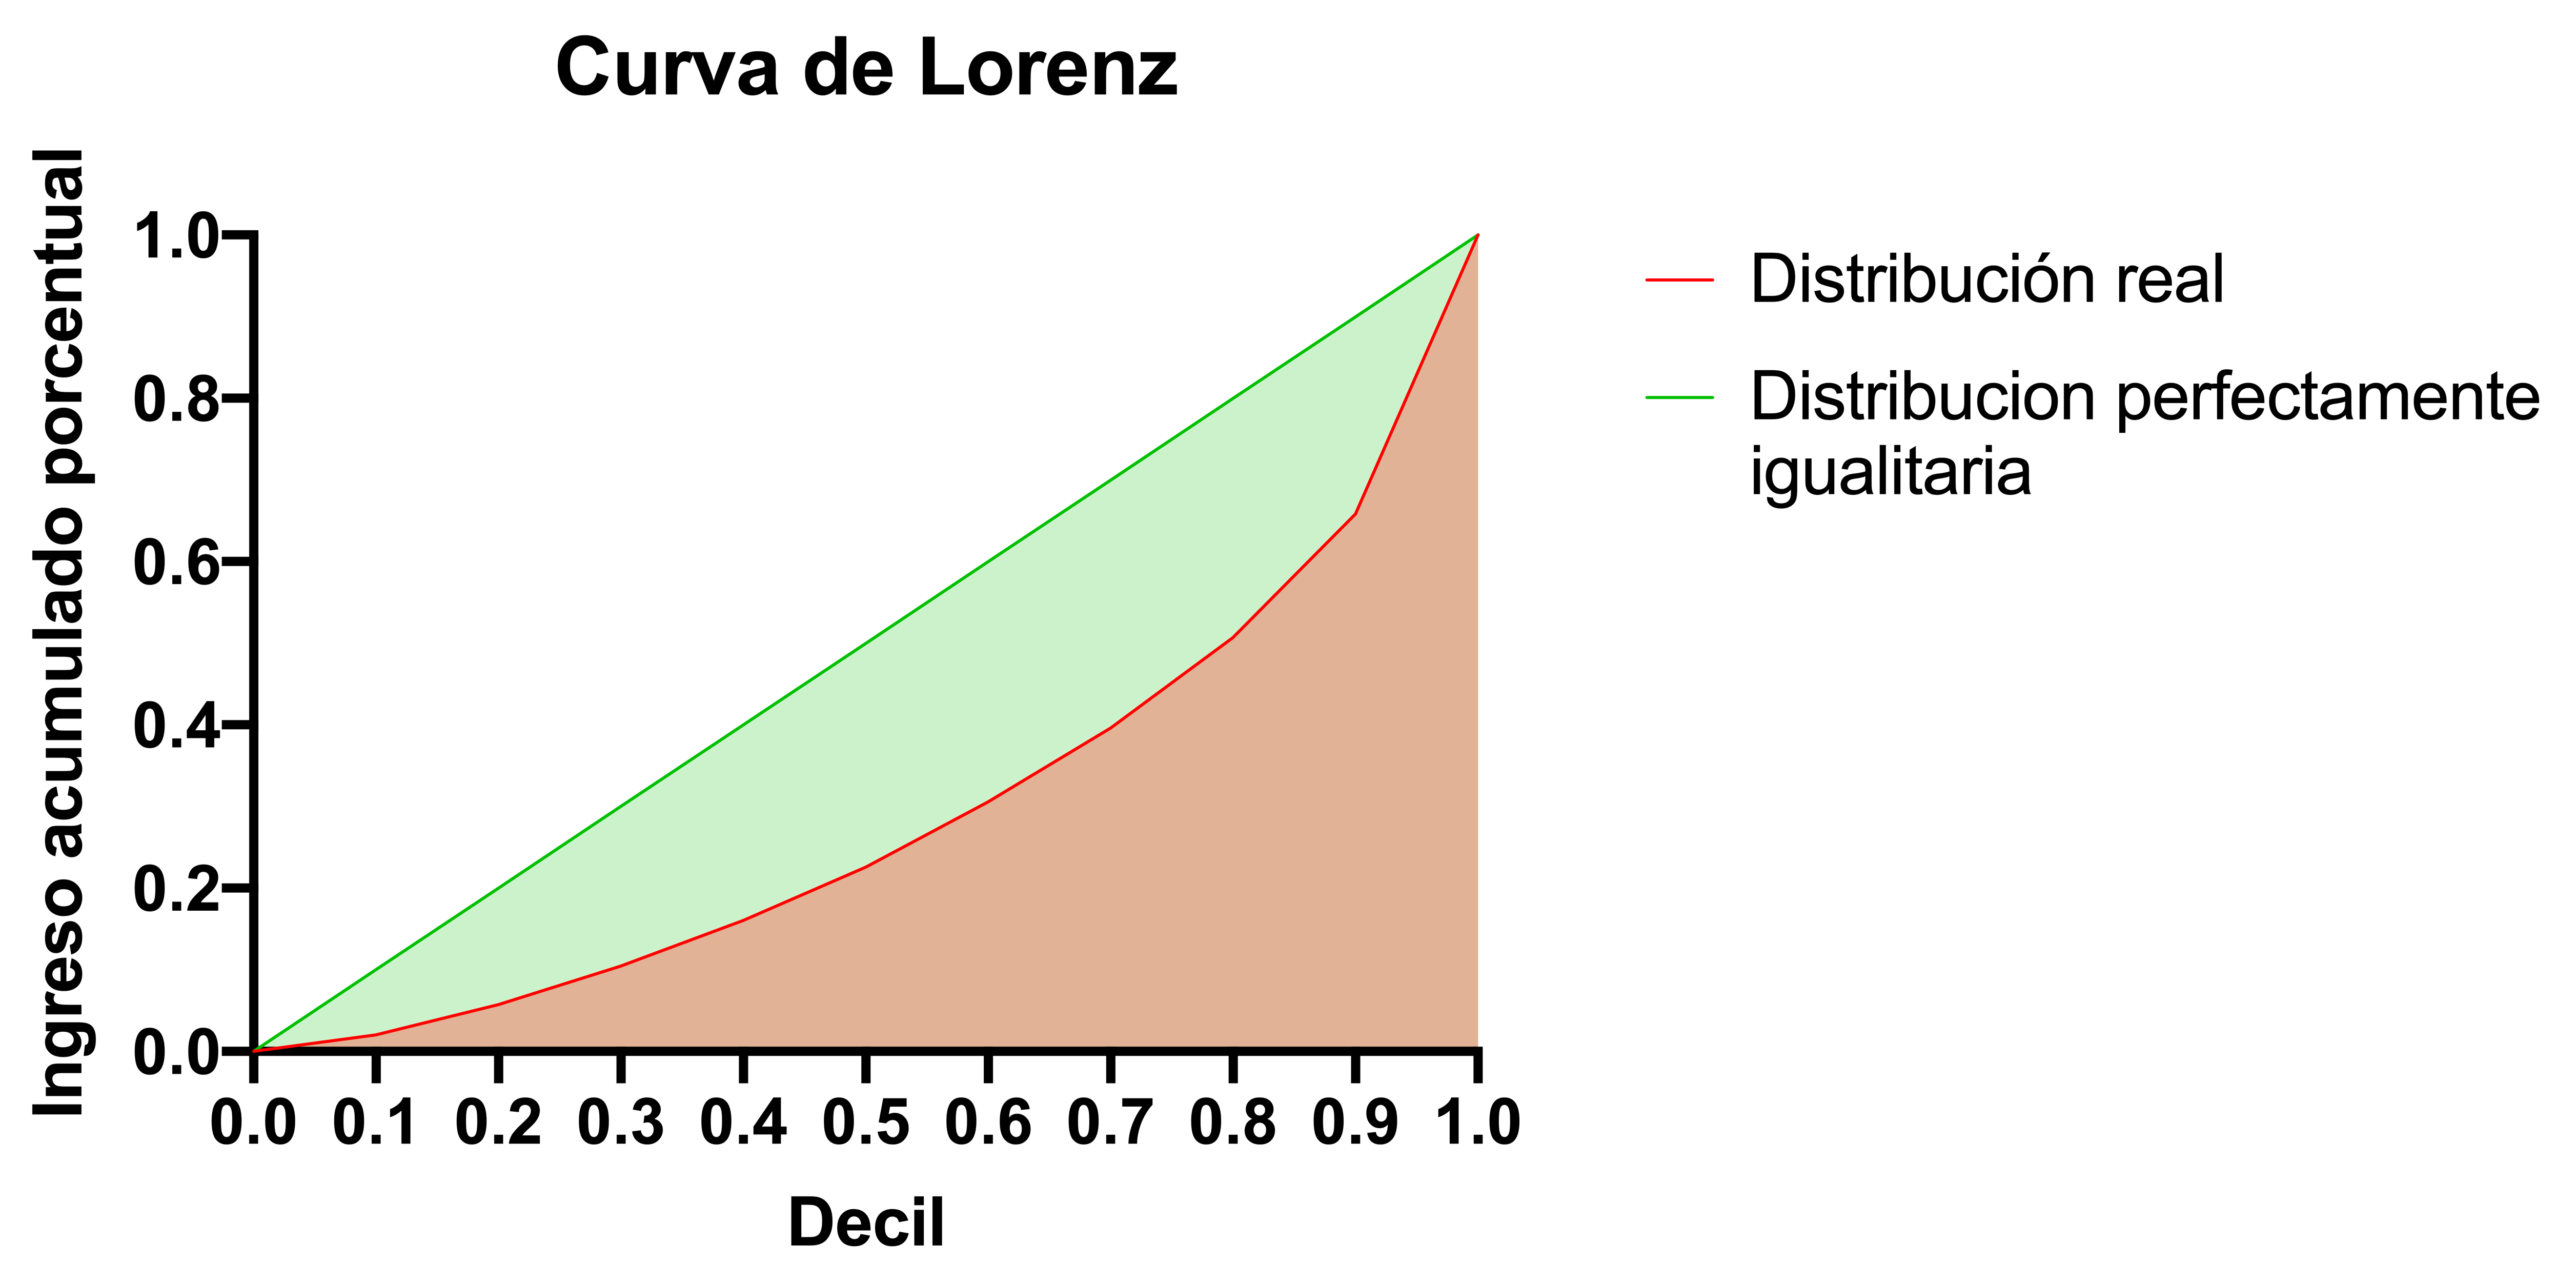
\includegraphics[width=0.84\textwidth]{Modulo_4/Curva_Lorenz_Final.png}
    \caption{Curva de Lorenz correspondiente a Chile, Casen 2017}
    \label{fig:lorenz_casen_2017}
\end{figure}

La figura \ref{fig:lorenz_casen_2017} muestra la curva de Lorenz correspondiente a Chile según la encuesta Casen 2017. En esta se puede observar en el eje vertical el \textit{Ingreso acumulado porcentual} y en el eje horizontal el \textit{Decil correspondiente} donde $0.1$ corresponde al decil 1, y así sucesivamente. \hfill \break


El índice de Gini se puede calcular a partir de las áreas bajo la curva del gráfico. Dividiendo el área entre la curva de la DPI y la distribución real, y sobre el área total. 
\[G = \frac{A_{DPI} - A_{DR}}{A_{total}}\]


En el caso de la figura \ref{fig:lorenz_casen_2017}, correspondería a dividir el área verde sobre la suma de las áreas verde y naranja. 
\newpage
\section{Criterios de asignación}

\econ{https://www.core-econ.org/the-economy/book/es/text/05.html}{5}

\subsection{Criterios de asignación}
Se entiende una asignación como el resultado de un determinado proceso económico.

\subsection{Eficiencia de Pareto}
Sean $A$ y $B$ asignaciones, la eficiencia de pareto establece que:
\hfill \break
\hfill \break
\textit{La asignación $A$ prevalece sobre la asignación $B$, si al menos una de las partes estaría mejor con $A$ que con $B$, y nadie estaría peor. En este caso $A$ domina a $B$ en términos de Pareto.}
\hfill \break


Una asignación que no está dominada en términos de Pareto se denomina \textbf{Pareto-eficiente.}


Este criterio es lo que en matemáticas se conoce como un orden parcial. Es decir, permite ordenar algunas asignaciones, pero no todas (esto sería un orden completo).

\subsubsection{Comentarios sobre la eficiencia de Pareto}
El criterio de la eficiencia de Pareto es uno de los conceptos más relevantes en economía. 


Dado un problema determinado, pueden existir muchas asignaciones que son pareto-eficientes. Pero sin un criterio adicional, no podemos decir cual de ellas es preferible.


Que una asignación sea eficiente de Pareto, no significa que estemos de acuerdo con ella. De hecho, si se le entregara todo el ingreso a una persona en la sociedad y dejamos a todo el resto sin nada, esa asignación es Pareto-Eficiente, pero probablemente no estemos de acuerdo en que sea una buena asignación económica.


Además, en muchas ocasiones, existe más de una asignación eficiente en términos de Pareto.

\subsection{Asignaciones}
Existen distintos casos posibles, y según este la manera de calcular asignación óptima varía.


\href{https://www.youtube.com/watch?v=jWcbHlTCPnQ}{Video EOL}
\begin{enumerate}[label=\Roman*.]
    \item \textbf{La persona genera el bien por si misma} \textit{(\href{https://youtu.be/jWcbHlTCPnQ?t=64}{Min 1:04})}, aquí $TMS = TMT$ es la condición de asignación óptima. 
    
    \item \textbf{Coerción} \textit{(\href{https://youtu.be/jWcbHlTCPnQ?t=181}{Min 3:01})}: alguien obliga a la persona a trabajar y se queda con los excedentes luego de darle lo mínimo que necesita la persona para subsistir (esclavitud). Existe una \textit{restricción de supervivencia biológica (RSB)}.
    
    El coerzor escogerá el punto donde la distancia entre la frontera del conjunto factible y la curva de RSB sea mayor.\\
    
    $TMB = TMT$ es la asignación óptima. (TMB es la tasa relacionada con RSB)
    
    \item \textbf{Propiedad privada} \textit{(\href{https://youtu.be/jWcbHlTCPnQ?t=333}{Min 5:33})}: La otra persona tiene todo el poder de negociación pero la primera persona solo trabajará si obtiene ganancias. \\
    
    Alguien externo (e.g. Estado o familia) ofrece una producción de sobrevivencia.\\
    
    Existe una curva de indiferencia de la primera persona. Se busca maximizar la distancia entre esa curva y la frontera factible.\\
    
    $TMT = TMS$ es la condición de optimalidad.
    
    \item \textbf{Negociación colectiva} \textit{(\href{https://youtu.be/jWcbHlTCPnQ?t=510}{Min 8:30})}: La primera persona busca parte del excedente.\\
    
    Una \hyperlink{institucion}{institución} externa (e.g. Estado) establece una curva de indiferencia nueva que ha de cumplirse, no necesariamente es Pareto-eficiente.\\
    
    A la persona se le puede ofrecer una nueva curva de indiferencia que le deje con igual igual utilidad (y que cumpla lo propuesto por el Estado) o que deje a ambas partes mejor.\\
    
    $TMT = TMS$ es la condición de optimalidad.
\end{enumerate}

\subsection{Desigualdad (criterios)}
Existen distintos tipos de medida a la hora de medir desigualdad, entre estas están

\begin{itemize}
    \item \textbf{Desigualdad absoluta}: es la resta de ingresos. Posee un problema que es que posee unidades dimensionales de ingreso lo cual hace difícil comparar entre lugares que no poseen las mismas unidades monetarias. Además aumenta cuando el país crece, aunque ambos ingresos crezcan a la misma \textit{tasa}. $\quad DA = Y_R - Y_P$
    
    \item \textbf{Desigualdad relativa}: es la división entre los ingresos. Es adimensional y no aumenta trivialmente cuando el país crece. $\quad DR = Y_R/Y_P$
\end{itemize}

Por esto es preferible hacer uso de la desigualdad relativa.

\subsubsection{Razones o \textit{ratios} de desigualdad}
Es la medida más sencilla de desigualdad, es la razón entre los ingresos de los sectores más ricos y pobres de la sociedad.

\begin{itemize}
    \item Razones entre quintiles
    \item Razones entre deciles
\end{itemize}

\subsubsection{Razón o índice de Palma}
Es un refinamiento de los \textit{ratios}, este índice considera que hay 3 grupos en la sociedad
\begin{enumerate}[label=\arabic*)]
    \item Los ricos (decil 10)
    \item Clase media (Decil 5 a 9)
    \item Los pobres (Decil 1 a 4)
\end{enumerate}

Se sustenta con la observación empírica: la clase media tiende a capturar la mitad del ingreso. 

\[\text{Razón de palma} = \frac{D_{10}}{D_1+D_2+D_3+D_4}\]

\subsubsection{Coeficiente o índice de Gini}
Es la medida más usada de desigualdad, representa que tanto se aleja una distribución real de una distribución totalmente igualitaria. Su valor varía entre 0 y 1, siendo mínima la desigualdad en 0 y máxima en 1. Posee dos formas:

\begin{enumerate}[label=\roman*.]
    \item \textbf{Forma general}: promedio de las diferencias de ingreso entre todos los individuos en una economía. Se calcula como \newline
    \[G = \frac{\sum_i\sum_j\abs{y_i-y_j}}{2\sum_{ij}y_i}\]
    
    \item \textbf{Forma de Sen}: suma ponderada de ingresos. (más usada)
    \newline
    \[G = \frac{2}{n}\frac{\sum_i^n i y_i}{\sum_i^n y_i} - \frac{n+1}{n}\]
\end{enumerate}


Donde $y_i$ son los ingresos correspondientes a $i$, e $i$ pueden ser deciles, quintiles, personas, etc. de las que hay una cantidad $n$.
\\

La interpretación más usual del coeficiente de Gini es a partir de la curva de Lorenz.
\subsubsection{Curva de Lorenz}
Muestra los ingresos acumulados desde los individuos más pobres a los más ricos de la sociedad. Comparándolos con la curva correspondiente a una distribución perfectamente igualitaria (DPI).

\begin{figure}[H]
    \centering
    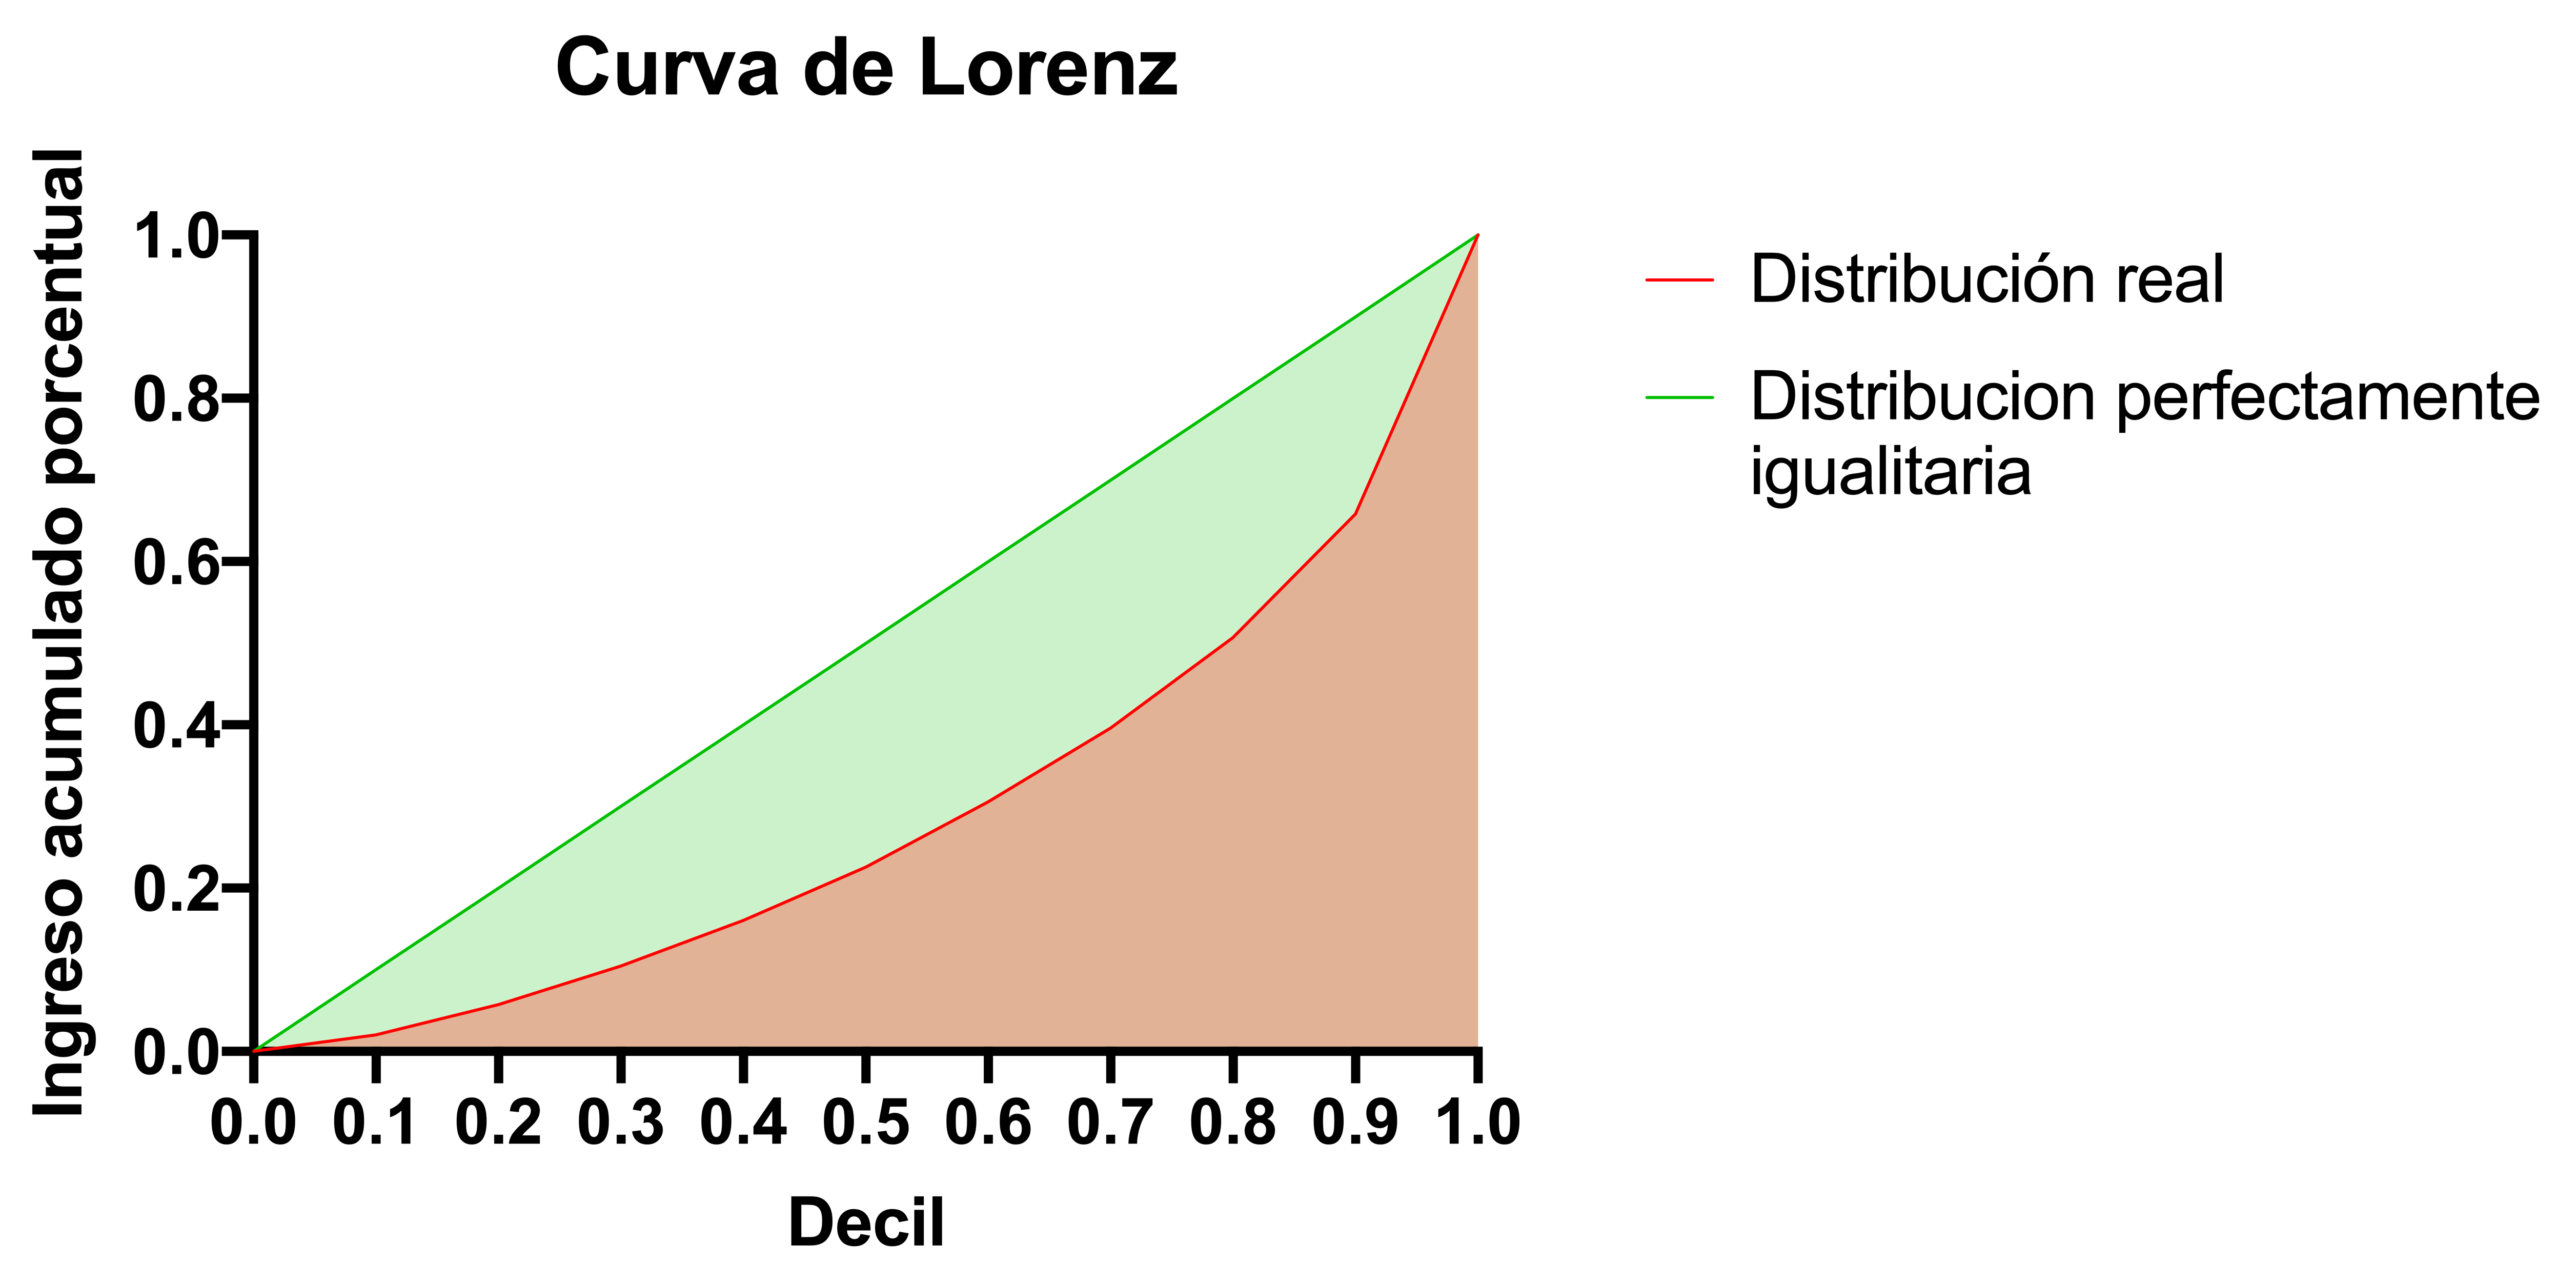
\includegraphics[width=0.84\textwidth]{Modulo_4/Curva_Lorenz_Final.png}
    \caption{Curva de Lorenz correspondiente a Chile, Casen 2017}
    \label{fig:lorenz_casen_2017}
\end{figure}

La figura \ref{fig:lorenz_casen_2017} muestra la curva de Lorenz correspondiente a Chile según la encuesta Casen 2017. En esta se puede observar en el eje vertical el \textit{Ingreso acumulado porcentual} y en el eje horizontal el \textit{Decil correspondiente} donde $0.1$ corresponde al decil 1, y así sucesivamente. \hfill \break


El índice de Gini se puede calcular a partir de las áreas bajo la curva del gráfico. Dividiendo el área entre la curva de la DPI y la distribución real, y sobre el área total. 
\[G = \frac{A_{DPI} - A_{DR}}{A_{total}}\]


En el caso de la figura \ref{fig:lorenz_casen_2017}, correspondería a dividir el área verde sobre la suma de las áreas verde y naranja. 
\newpage
\section{Criterios de asignación}

\econ{https://www.core-econ.org/the-economy/book/es/text/05.html}{5}

\subsection{Criterios de asignación}
Se entiende una asignación como el resultado de un determinado proceso económico.

\subsection{Eficiencia de Pareto}
Sean $A$ y $B$ asignaciones, la eficiencia de pareto establece que:
\hfill \break
\hfill \break
\textit{La asignación $A$ prevalece sobre la asignación $B$, si al menos una de las partes estaría mejor con $A$ que con $B$, y nadie estaría peor. En este caso $A$ domina a $B$ en términos de Pareto.}
\hfill \break


Una asignación que no está dominada en términos de Pareto se denomina \textbf{Pareto-eficiente.}


Este criterio es lo que en matemáticas se conoce como un orden parcial. Es decir, permite ordenar algunas asignaciones, pero no todas (esto sería un orden completo).

\subsubsection{Comentarios sobre la eficiencia de Pareto}
El criterio de la eficiencia de Pareto es uno de los conceptos más relevantes en economía. 


Dado un problema determinado, pueden existir muchas asignaciones que son pareto-eficientes. Pero sin un criterio adicional, no podemos decir cual de ellas es preferible.


Que una asignación sea eficiente de Pareto, no significa que estemos de acuerdo con ella. De hecho, si se le entregara todo el ingreso a una persona en la sociedad y dejamos a todo el resto sin nada, esa asignación es Pareto-Eficiente, pero probablemente no estemos de acuerdo en que sea una buena asignación económica.


Además, en muchas ocasiones, existe más de una asignación eficiente en términos de Pareto.

\subsection{Asignaciones}
Existen distintos casos posibles, y según este la manera de calcular asignación óptima varía.


\href{https://www.youtube.com/watch?v=jWcbHlTCPnQ}{Video EOL}
\begin{enumerate}[label=\Roman*.]
    \item \textbf{La persona genera el bien por si misma} \textit{(\href{https://youtu.be/jWcbHlTCPnQ?t=64}{Min 1:04})}, aquí $TMS = TMT$ es la condición de asignación óptima. 
    
    \item \textbf{Coerción} \textit{(\href{https://youtu.be/jWcbHlTCPnQ?t=181}{Min 3:01})}: alguien obliga a la persona a trabajar y se queda con los excedentes luego de darle lo mínimo que necesita la persona para subsistir (esclavitud). Existe una \textit{restricción de supervivencia biológica (RSB)}.
    
    El coerzor escogerá el punto donde la distancia entre la frontera del conjunto factible y la curva de RSB sea mayor.\\
    
    $TMB = TMT$ es la asignación óptima. (TMB es la tasa relacionada con RSB)
    
    \item \textbf{Propiedad privada} \textit{(\href{https://youtu.be/jWcbHlTCPnQ?t=333}{Min 5:33})}: La otra persona tiene todo el poder de negociación pero la primera persona solo trabajará si obtiene ganancias. \\
    
    Alguien externo (e.g. Estado o familia) ofrece una producción de sobrevivencia.\\
    
    Existe una curva de indiferencia de la primera persona. Se busca maximizar la distancia entre esa curva y la frontera factible.\\
    
    $TMT = TMS$ es la condición de optimalidad.
    
    \item \textbf{Negociación colectiva} \textit{(\href{https://youtu.be/jWcbHlTCPnQ?t=510}{Min 8:30})}: La primera persona busca parte del excedente.\\
    
    Una \hyperlink{institucion}{institución} externa (e.g. Estado) establece una curva de indiferencia nueva que ha de cumplirse, no necesariamente es Pareto-eficiente.\\
    
    A la persona se le puede ofrecer una nueva curva de indiferencia que le deje con igual igual utilidad (y que cumpla lo propuesto por el Estado) o que deje a ambas partes mejor.\\
    
    $TMT = TMS$ es la condición de optimalidad.
\end{enumerate}

\subsection{Desigualdad (criterios)}
Existen distintos tipos de medida a la hora de medir desigualdad, entre estas están

\begin{itemize}
    \item \textbf{Desigualdad absoluta}: es la resta de ingresos. Posee un problema que es que posee unidades dimensionales de ingreso lo cual hace difícil comparar entre lugares que no poseen las mismas unidades monetarias. Además aumenta cuando el país crece, aunque ambos ingresos crezcan a la misma \textit{tasa}. $\quad DA = Y_R - Y_P$
    
    \item \textbf{Desigualdad relativa}: es la división entre los ingresos. Es adimensional y no aumenta trivialmente cuando el país crece. $\quad DR = Y_R/Y_P$
\end{itemize}

Por esto es preferible hacer uso de la desigualdad relativa.

\subsubsection{Razones o \textit{ratios} de desigualdad}
Es la medida más sencilla de desigualdad, es la razón entre los ingresos de los sectores más ricos y pobres de la sociedad.

\begin{itemize}
    \item Razones entre quintiles
    \item Razones entre deciles
\end{itemize}

\subsubsection{Razón o índice de Palma}
Es un refinamiento de los \textit{ratios}, este índice considera que hay 3 grupos en la sociedad
\begin{enumerate}[label=\arabic*)]
    \item Los ricos (decil 10)
    \item Clase media (Decil 5 a 9)
    \item Los pobres (Decil 1 a 4)
\end{enumerate}

Se sustenta con la observación empírica: la clase media tiende a capturar la mitad del ingreso. 

\[\text{Razón de palma} = \frac{D_{10}}{D_1+D_2+D_3+D_4}\]

\subsubsection{Coeficiente o índice de Gini}
Es la medida más usada de desigualdad, representa que tanto se aleja una distribución real de una distribución totalmente igualitaria. Su valor varía entre 0 y 1, siendo mínima la desigualdad en 0 y máxima en 1. Posee dos formas:

\begin{enumerate}[label=\roman*.]
    \item \textbf{Forma general}: promedio de las diferencias de ingreso entre todos los individuos en una economía. Se calcula como \newline
    \[G = \frac{\sum_i\sum_j\abs{y_i-y_j}}{2\sum_{ij}y_i}\]
    
    \item \textbf{Forma de Sen}: suma ponderada de ingresos. (más usada)
    \newline
    \[G = \frac{2}{n}\frac{\sum_i^n i y_i}{\sum_i^n y_i} - \frac{n+1}{n}\]
\end{enumerate}


Donde $y_i$ son los ingresos correspondientes a $i$, e $i$ pueden ser deciles, quintiles, personas, etc. de las que hay una cantidad $n$.
\\

La interpretación más usual del coeficiente de Gini es a partir de la curva de Lorenz.
\subsubsection{Curva de Lorenz}
Muestra los ingresos acumulados desde los individuos más pobres a los más ricos de la sociedad. Comparándolos con la curva correspondiente a una distribución perfectamente igualitaria (DPI).

\begin{figure}[H]
    \centering
    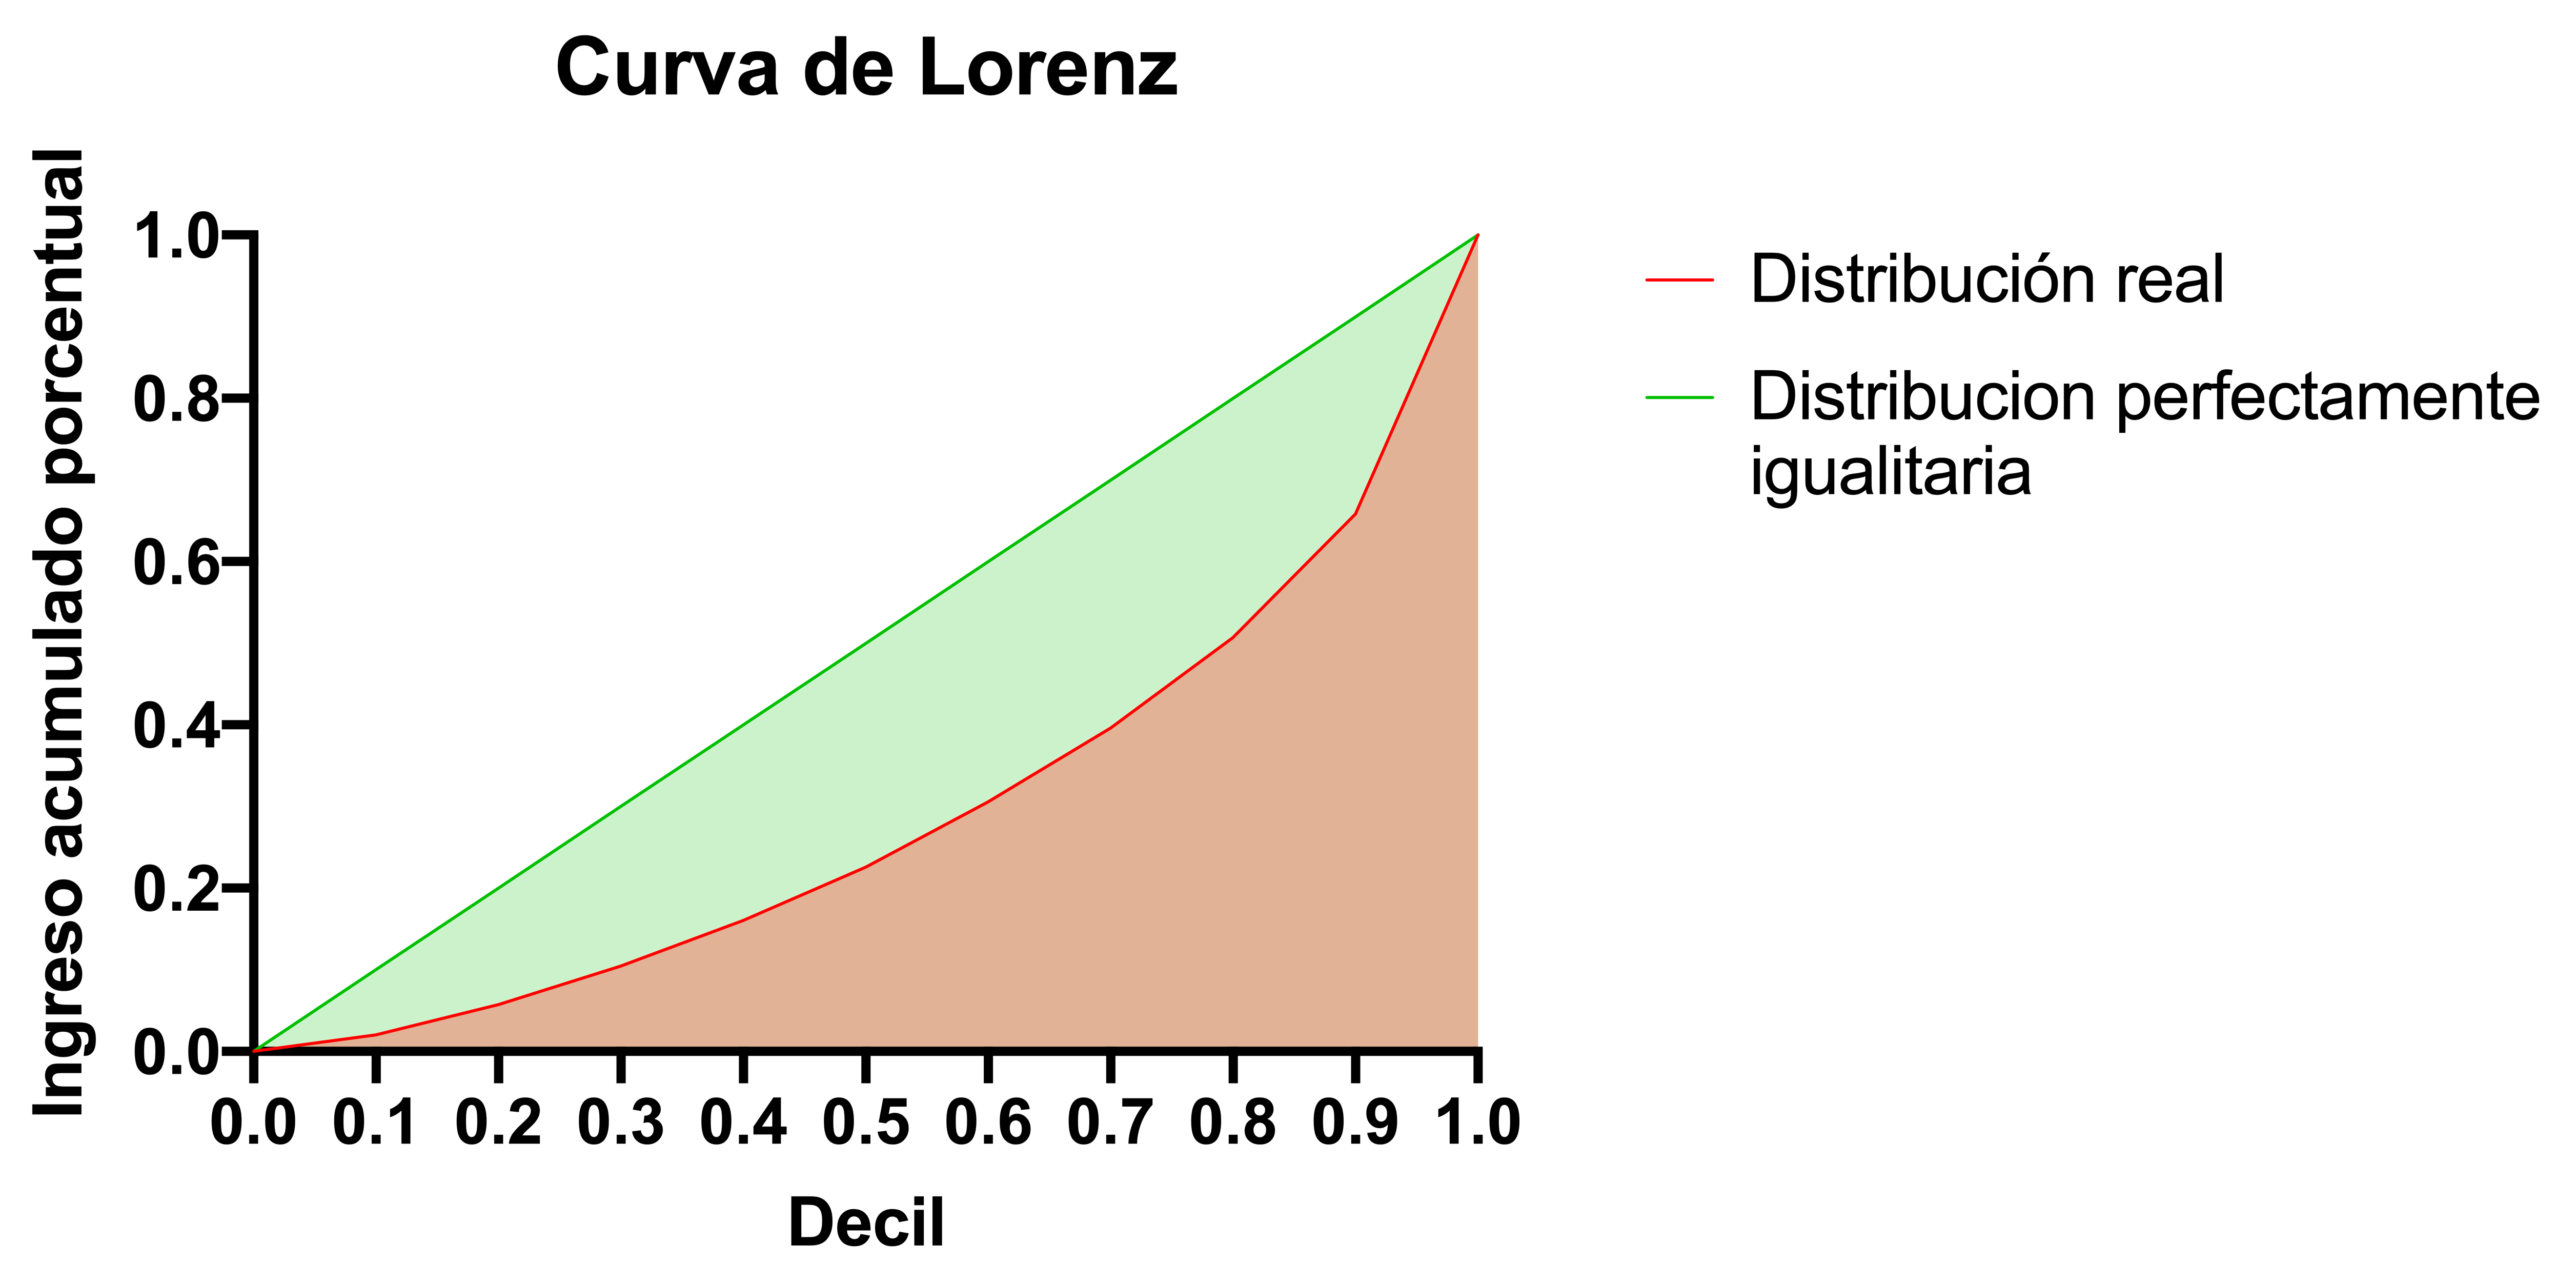
\includegraphics[width=0.84\textwidth]{Modulo_4/Curva_Lorenz_Final.png}
    \caption{Curva de Lorenz correspondiente a Chile, Casen 2017}
    \label{fig:lorenz_casen_2017}
\end{figure}

La figura \ref{fig:lorenz_casen_2017} muestra la curva de Lorenz correspondiente a Chile según la encuesta Casen 2017. En esta se puede observar en el eje vertical el \textit{Ingreso acumulado porcentual} y en el eje horizontal el \textit{Decil correspondiente} donde $0.1$ corresponde al decil 1, y así sucesivamente. \hfill \break


El índice de Gini se puede calcular a partir de las áreas bajo la curva del gráfico. Dividiendo el área entre la curva de la DPI y la distribución real, y sobre el área total. 
\[G = \frac{A_{DPI} - A_{DR}}{A_{total}}\]


En el caso de la figura \ref{fig:lorenz_casen_2017}, correspondería a dividir el área verde sobre la suma de las áreas verde y naranja. 
\newpage
\section{Criterios de asignación}

\econ{https://www.core-econ.org/the-economy/book/es/text/05.html}{5}

\subsection{Criterios de asignación}
Se entiende una asignación como el resultado de un determinado proceso económico.

\subsection{Eficiencia de Pareto}
Sean $A$ y $B$ asignaciones, la eficiencia de pareto establece que:
\hfill \break
\hfill \break
\textit{La asignación $A$ prevalece sobre la asignación $B$, si al menos una de las partes estaría mejor con $A$ que con $B$, y nadie estaría peor. En este caso $A$ domina a $B$ en términos de Pareto.}
\hfill \break


Una asignación que no está dominada en términos de Pareto se denomina \textbf{Pareto-eficiente.}


Este criterio es lo que en matemáticas se conoce como un orden parcial. Es decir, permite ordenar algunas asignaciones, pero no todas (esto sería un orden completo).

\subsubsection{Comentarios sobre la eficiencia de Pareto}
El criterio de la eficiencia de Pareto es uno de los conceptos más relevantes en economía. 


Dado un problema determinado, pueden existir muchas asignaciones que son pareto-eficientes. Pero sin un criterio adicional, no podemos decir cual de ellas es preferible.


Que una asignación sea eficiente de Pareto, no significa que estemos de acuerdo con ella. De hecho, si se le entregara todo el ingreso a una persona en la sociedad y dejamos a todo el resto sin nada, esa asignación es Pareto-Eficiente, pero probablemente no estemos de acuerdo en que sea una buena asignación económica.


Además, en muchas ocasiones, existe más de una asignación eficiente en términos de Pareto.

\subsection{Asignaciones}
Existen distintos casos posibles, y según este la manera de calcular asignación óptima varía.


\href{https://www.youtube.com/watch?v=jWcbHlTCPnQ}{Video EOL}
\begin{enumerate}[label=\Roman*.]
    \item \textbf{La persona genera el bien por si misma} \textit{(\href{https://youtu.be/jWcbHlTCPnQ?t=64}{Min 1:04})}, aquí $TMS = TMT$ es la condición de asignación óptima. 
    
    \item \textbf{Coerción} \textit{(\href{https://youtu.be/jWcbHlTCPnQ?t=181}{Min 3:01})}: alguien obliga a la persona a trabajar y se queda con los excedentes luego de darle lo mínimo que necesita la persona para subsistir (esclavitud). Existe una \textit{restricción de supervivencia biológica (RSB)}.
    
    El coerzor escogerá el punto donde la distancia entre la frontera del conjunto factible y la curva de RSB sea mayor.\\
    
    $TMB = TMT$ es la asignación óptima. (TMB es la tasa relacionada con RSB)
    
    \item \textbf{Propiedad privada} \textit{(\href{https://youtu.be/jWcbHlTCPnQ?t=333}{Min 5:33})}: La otra persona tiene todo el poder de negociación pero la primera persona solo trabajará si obtiene ganancias. \\
    
    Alguien externo (e.g. Estado o familia) ofrece una producción de sobrevivencia.\\
    
    Existe una curva de indiferencia de la primera persona. Se busca maximizar la distancia entre esa curva y la frontera factible.\\
    
    $TMT = TMS$ es la condición de optimalidad.
    
    \item \textbf{Negociación colectiva} \textit{(\href{https://youtu.be/jWcbHlTCPnQ?t=510}{Min 8:30})}: La primera persona busca parte del excedente.\\
    
    Una \hyperlink{institucion}{institución} externa (e.g. Estado) establece una curva de indiferencia nueva que ha de cumplirse, no necesariamente es Pareto-eficiente.\\
    
    A la persona se le puede ofrecer una nueva curva de indiferencia que le deje con igual igual utilidad (y que cumpla lo propuesto por el Estado) o que deje a ambas partes mejor.\\
    
    $TMT = TMS$ es la condición de optimalidad.
\end{enumerate}

\subsection{Desigualdad (criterios)}
Existen distintos tipos de medida a la hora de medir desigualdad, entre estas están

\begin{itemize}
    \item \textbf{Desigualdad absoluta}: es la resta de ingresos. Posee un problema que es que posee unidades dimensionales de ingreso lo cual hace difícil comparar entre lugares que no poseen las mismas unidades monetarias. Además aumenta cuando el país crece, aunque ambos ingresos crezcan a la misma \textit{tasa}. $\quad DA = Y_R - Y_P$
    
    \item \textbf{Desigualdad relativa}: es la división entre los ingresos. Es adimensional y no aumenta trivialmente cuando el país crece. $\quad DR = Y_R/Y_P$
\end{itemize}

Por esto es preferible hacer uso de la desigualdad relativa.

\subsubsection{Razones o \textit{ratios} de desigualdad}
Es la medida más sencilla de desigualdad, es la razón entre los ingresos de los sectores más ricos y pobres de la sociedad.

\begin{itemize}
    \item Razones entre quintiles
    \item Razones entre deciles
\end{itemize}

\subsubsection{Razón o índice de Palma}
Es un refinamiento de los \textit{ratios}, este índice considera que hay 3 grupos en la sociedad
\begin{enumerate}[label=\arabic*)]
    \item Los ricos (decil 10)
    \item Clase media (Decil 5 a 9)
    \item Los pobres (Decil 1 a 4)
\end{enumerate}

Se sustenta con la observación empírica: la clase media tiende a capturar la mitad del ingreso. 

\[\text{Razón de palma} = \frac{D_{10}}{D_1+D_2+D_3+D_4}\]

\subsubsection{Coeficiente o índice de Gini}
Es la medida más usada de desigualdad, representa que tanto se aleja una distribución real de una distribución totalmente igualitaria. Su valor varía entre 0 y 1, siendo mínima la desigualdad en 0 y máxima en 1. Posee dos formas:

\begin{enumerate}[label=\roman*.]
    \item \textbf{Forma general}: promedio de las diferencias de ingreso entre todos los individuos en una economía. Se calcula como \newline
    \[G = \frac{\sum_i\sum_j\abs{y_i-y_j}}{2\sum_{ij}y_i}\]
    
    \item \textbf{Forma de Sen}: suma ponderada de ingresos. (más usada)
    \newline
    \[G = \frac{2}{n}\frac{\sum_i^n i y_i}{\sum_i^n y_i} - \frac{n+1}{n}\]
\end{enumerate}


Donde $y_i$ son los ingresos correspondientes a $i$, e $i$ pueden ser deciles, quintiles, personas, etc. de las que hay una cantidad $n$.
\\

La interpretación más usual del coeficiente de Gini es a partir de la curva de Lorenz.
\subsubsection{Curva de Lorenz}
Muestra los ingresos acumulados desde los individuos más pobres a los más ricos de la sociedad. Comparándolos con la curva correspondiente a una distribución perfectamente igualitaria (DPI).

\begin{figure}[H]
    \centering
    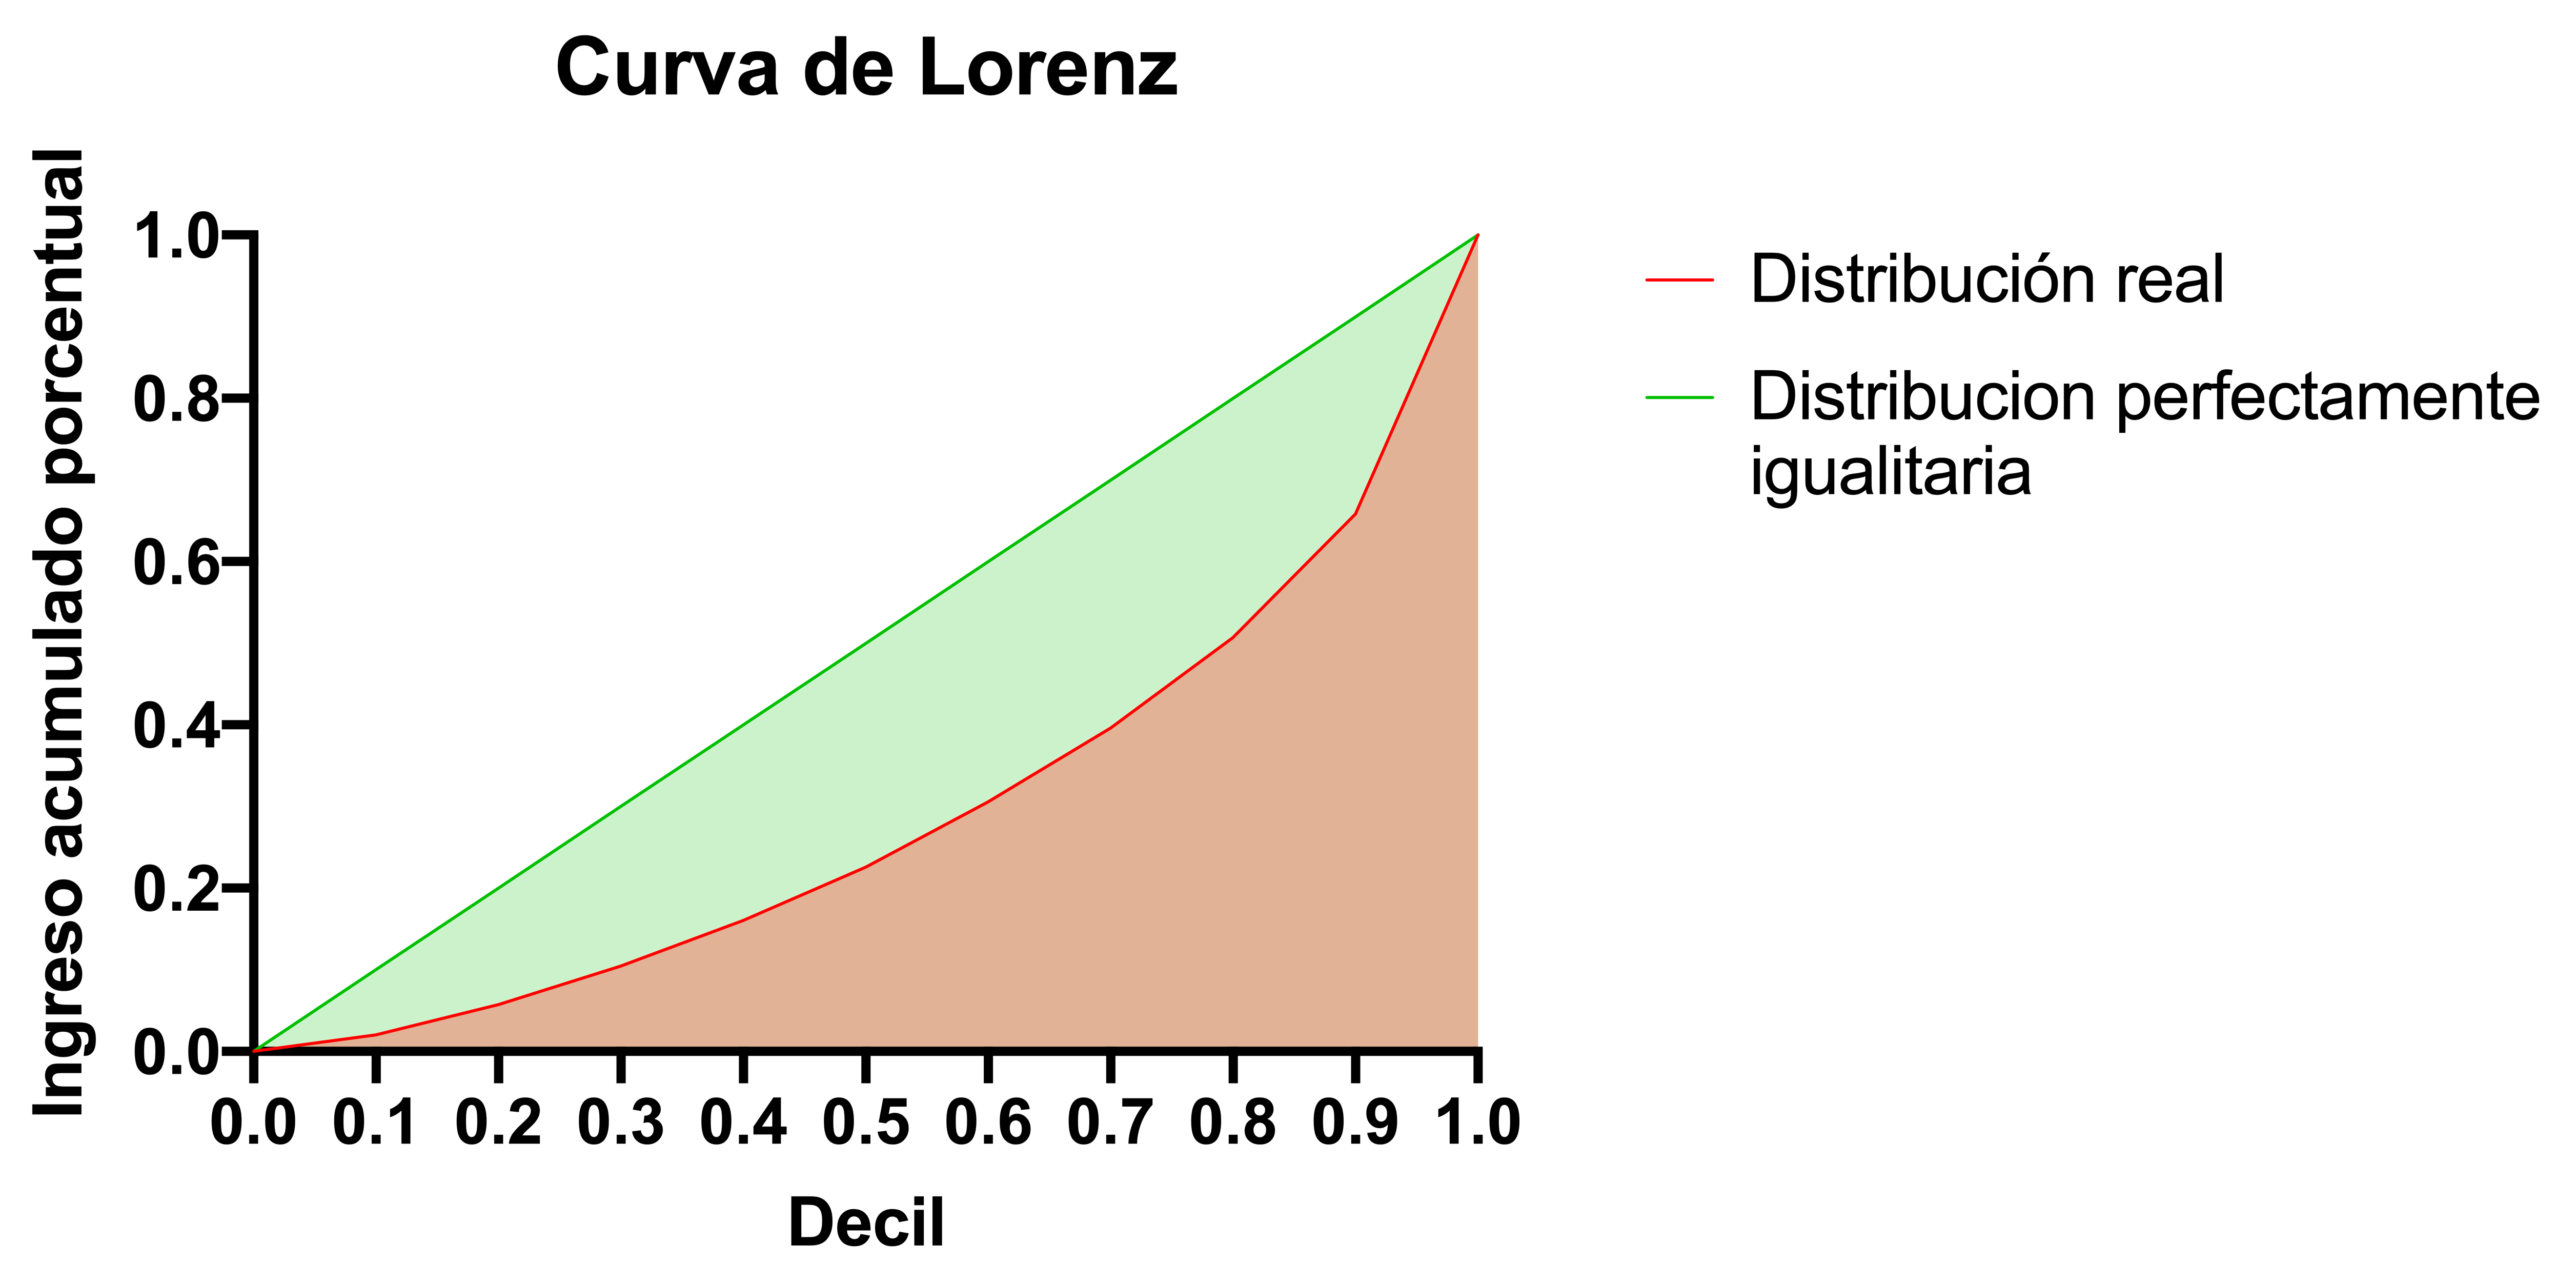
\includegraphics[width=0.84\textwidth]{Modulo_4/Curva_Lorenz_Final.png}
    \caption{Curva de Lorenz correspondiente a Chile, Casen 2017}
    \label{fig:lorenz_casen_2017}
\end{figure}

La figura \ref{fig:lorenz_casen_2017} muestra la curva de Lorenz correspondiente a Chile según la encuesta Casen 2017. En esta se puede observar en el eje vertical el \textit{Ingreso acumulado porcentual} y en el eje horizontal el \textit{Decil correspondiente} donde $0.1$ corresponde al decil 1, y así sucesivamente. \hfill \break


El índice de Gini se puede calcular a partir de las áreas bajo la curva del gráfico. Dividiendo el área entre la curva de la DPI y la distribución real, y sobre el área total. 
\[G = \frac{A_{DPI} - A_{DR}}{A_{total}}\]


En el caso de la figura \ref{fig:lorenz_casen_2017}, correspondería a dividir el área verde sobre la suma de las áreas verde y naranja. 
\newpage
\section{Criterios de asignación}

\econ{https://www.core-econ.org/the-economy/book/es/text/05.html}{5}

\subsection{Criterios de asignación}
Se entiende una asignación como el resultado de un determinado proceso económico.

\subsection{Eficiencia de Pareto}
Sean $A$ y $B$ asignaciones, la eficiencia de pareto establece que:
\hfill \break
\hfill \break
\textit{La asignación $A$ prevalece sobre la asignación $B$, si al menos una de las partes estaría mejor con $A$ que con $B$, y nadie estaría peor. En este caso $A$ domina a $B$ en términos de Pareto.}
\hfill \break


Una asignación que no está dominada en términos de Pareto se denomina \textbf{Pareto-eficiente.}


Este criterio es lo que en matemáticas se conoce como un orden parcial. Es decir, permite ordenar algunas asignaciones, pero no todas (esto sería un orden completo).

\subsubsection{Comentarios sobre la eficiencia de Pareto}
El criterio de la eficiencia de Pareto es uno de los conceptos más relevantes en economía. 


Dado un problema determinado, pueden existir muchas asignaciones que son pareto-eficientes. Pero sin un criterio adicional, no podemos decir cual de ellas es preferible.


Que una asignación sea eficiente de Pareto, no significa que estemos de acuerdo con ella. De hecho, si se le entregara todo el ingreso a una persona en la sociedad y dejamos a todo el resto sin nada, esa asignación es Pareto-Eficiente, pero probablemente no estemos de acuerdo en que sea una buena asignación económica.


Además, en muchas ocasiones, existe más de una asignación eficiente en términos de Pareto.

\subsection{Asignaciones}
Existen distintos casos posibles, y según este la manera de calcular asignación óptima varía.


\href{https://www.youtube.com/watch?v=jWcbHlTCPnQ}{Video EOL}
\begin{enumerate}[label=\Roman*.]
    \item \textbf{La persona genera el bien por si misma} \textit{(\href{https://youtu.be/jWcbHlTCPnQ?t=64}{Min 1:04})}, aquí $TMS = TMT$ es la condición de asignación óptima. 
    
    \item \textbf{Coerción} \textit{(\href{https://youtu.be/jWcbHlTCPnQ?t=181}{Min 3:01})}: alguien obliga a la persona a trabajar y se queda con los excedentes luego de darle lo mínimo que necesita la persona para subsistir (esclavitud). Existe una \textit{restricción de supervivencia biológica (RSB)}.
    
    El coerzor escogerá el punto donde la distancia entre la frontera del conjunto factible y la curva de RSB sea mayor.\\
    
    $TMB = TMT$ es la asignación óptima. (TMB es la tasa relacionada con RSB)
    
    \item \textbf{Propiedad privada} \textit{(\href{https://youtu.be/jWcbHlTCPnQ?t=333}{Min 5:33})}: La otra persona tiene todo el poder de negociación pero la primera persona solo trabajará si obtiene ganancias. \\
    
    Alguien externo (e.g. Estado o familia) ofrece una producción de sobrevivencia.\\
    
    Existe una curva de indiferencia de la primera persona. Se busca maximizar la distancia entre esa curva y la frontera factible.\\
    
    $TMT = TMS$ es la condición de optimalidad.
    
    \item \textbf{Negociación colectiva} \textit{(\href{https://youtu.be/jWcbHlTCPnQ?t=510}{Min 8:30})}: La primera persona busca parte del excedente.\\
    
    Una \hyperlink{institucion}{institución} externa (e.g. Estado) establece una curva de indiferencia nueva que ha de cumplirse, no necesariamente es Pareto-eficiente.\\
    
    A la persona se le puede ofrecer una nueva curva de indiferencia que le deje con igual igual utilidad (y que cumpla lo propuesto por el Estado) o que deje a ambas partes mejor.\\
    
    $TMT = TMS$ es la condición de optimalidad.
\end{enumerate}

\subsection{Desigualdad (criterios)}
Existen distintos tipos de medida a la hora de medir desigualdad, entre estas están

\begin{itemize}
    \item \textbf{Desigualdad absoluta}: es la resta de ingresos. Posee un problema que es que posee unidades dimensionales de ingreso lo cual hace difícil comparar entre lugares que no poseen las mismas unidades monetarias. Además aumenta cuando el país crece, aunque ambos ingresos crezcan a la misma \textit{tasa}. $\quad DA = Y_R - Y_P$
    
    \item \textbf{Desigualdad relativa}: es la división entre los ingresos. Es adimensional y no aumenta trivialmente cuando el país crece. $\quad DR = Y_R/Y_P$
\end{itemize}

Por esto es preferible hacer uso de la desigualdad relativa.

\subsubsection{Razones o \textit{ratios} de desigualdad}
Es la medida más sencilla de desigualdad, es la razón entre los ingresos de los sectores más ricos y pobres de la sociedad.

\begin{itemize}
    \item Razones entre quintiles
    \item Razones entre deciles
\end{itemize}

\subsubsection{Razón o índice de Palma}
Es un refinamiento de los \textit{ratios}, este índice considera que hay 3 grupos en la sociedad
\begin{enumerate}[label=\arabic*)]
    \item Los ricos (decil 10)
    \item Clase media (Decil 5 a 9)
    \item Los pobres (Decil 1 a 4)
\end{enumerate}

Se sustenta con la observación empírica: la clase media tiende a capturar la mitad del ingreso. 

\[\text{Razón de palma} = \frac{D_{10}}{D_1+D_2+D_3+D_4}\]

\subsubsection{Coeficiente o índice de Gini}
Es la medida más usada de desigualdad, representa que tanto se aleja una distribución real de una distribución totalmente igualitaria. Su valor varía entre 0 y 1, siendo mínima la desigualdad en 0 y máxima en 1. Posee dos formas:

\begin{enumerate}[label=\roman*.]
    \item \textbf{Forma general}: promedio de las diferencias de ingreso entre todos los individuos en una economía. Se calcula como \newline
    \[G = \frac{\sum_i\sum_j\abs{y_i-y_j}}{2\sum_{ij}y_i}\]
    
    \item \textbf{Forma de Sen}: suma ponderada de ingresos. (más usada)
    \newline
    \[G = \frac{2}{n}\frac{\sum_i^n i y_i}{\sum_i^n y_i} - \frac{n+1}{n}\]
\end{enumerate}


Donde $y_i$ son los ingresos correspondientes a $i$, e $i$ pueden ser deciles, quintiles, personas, etc. de las que hay una cantidad $n$.
\\

La interpretación más usual del coeficiente de Gini es a partir de la curva de Lorenz.
\subsubsection{Curva de Lorenz}
Muestra los ingresos acumulados desde los individuos más pobres a los más ricos de la sociedad. Comparándolos con la curva correspondiente a una distribución perfectamente igualitaria (DPI).

\begin{figure}[H]
    \centering
    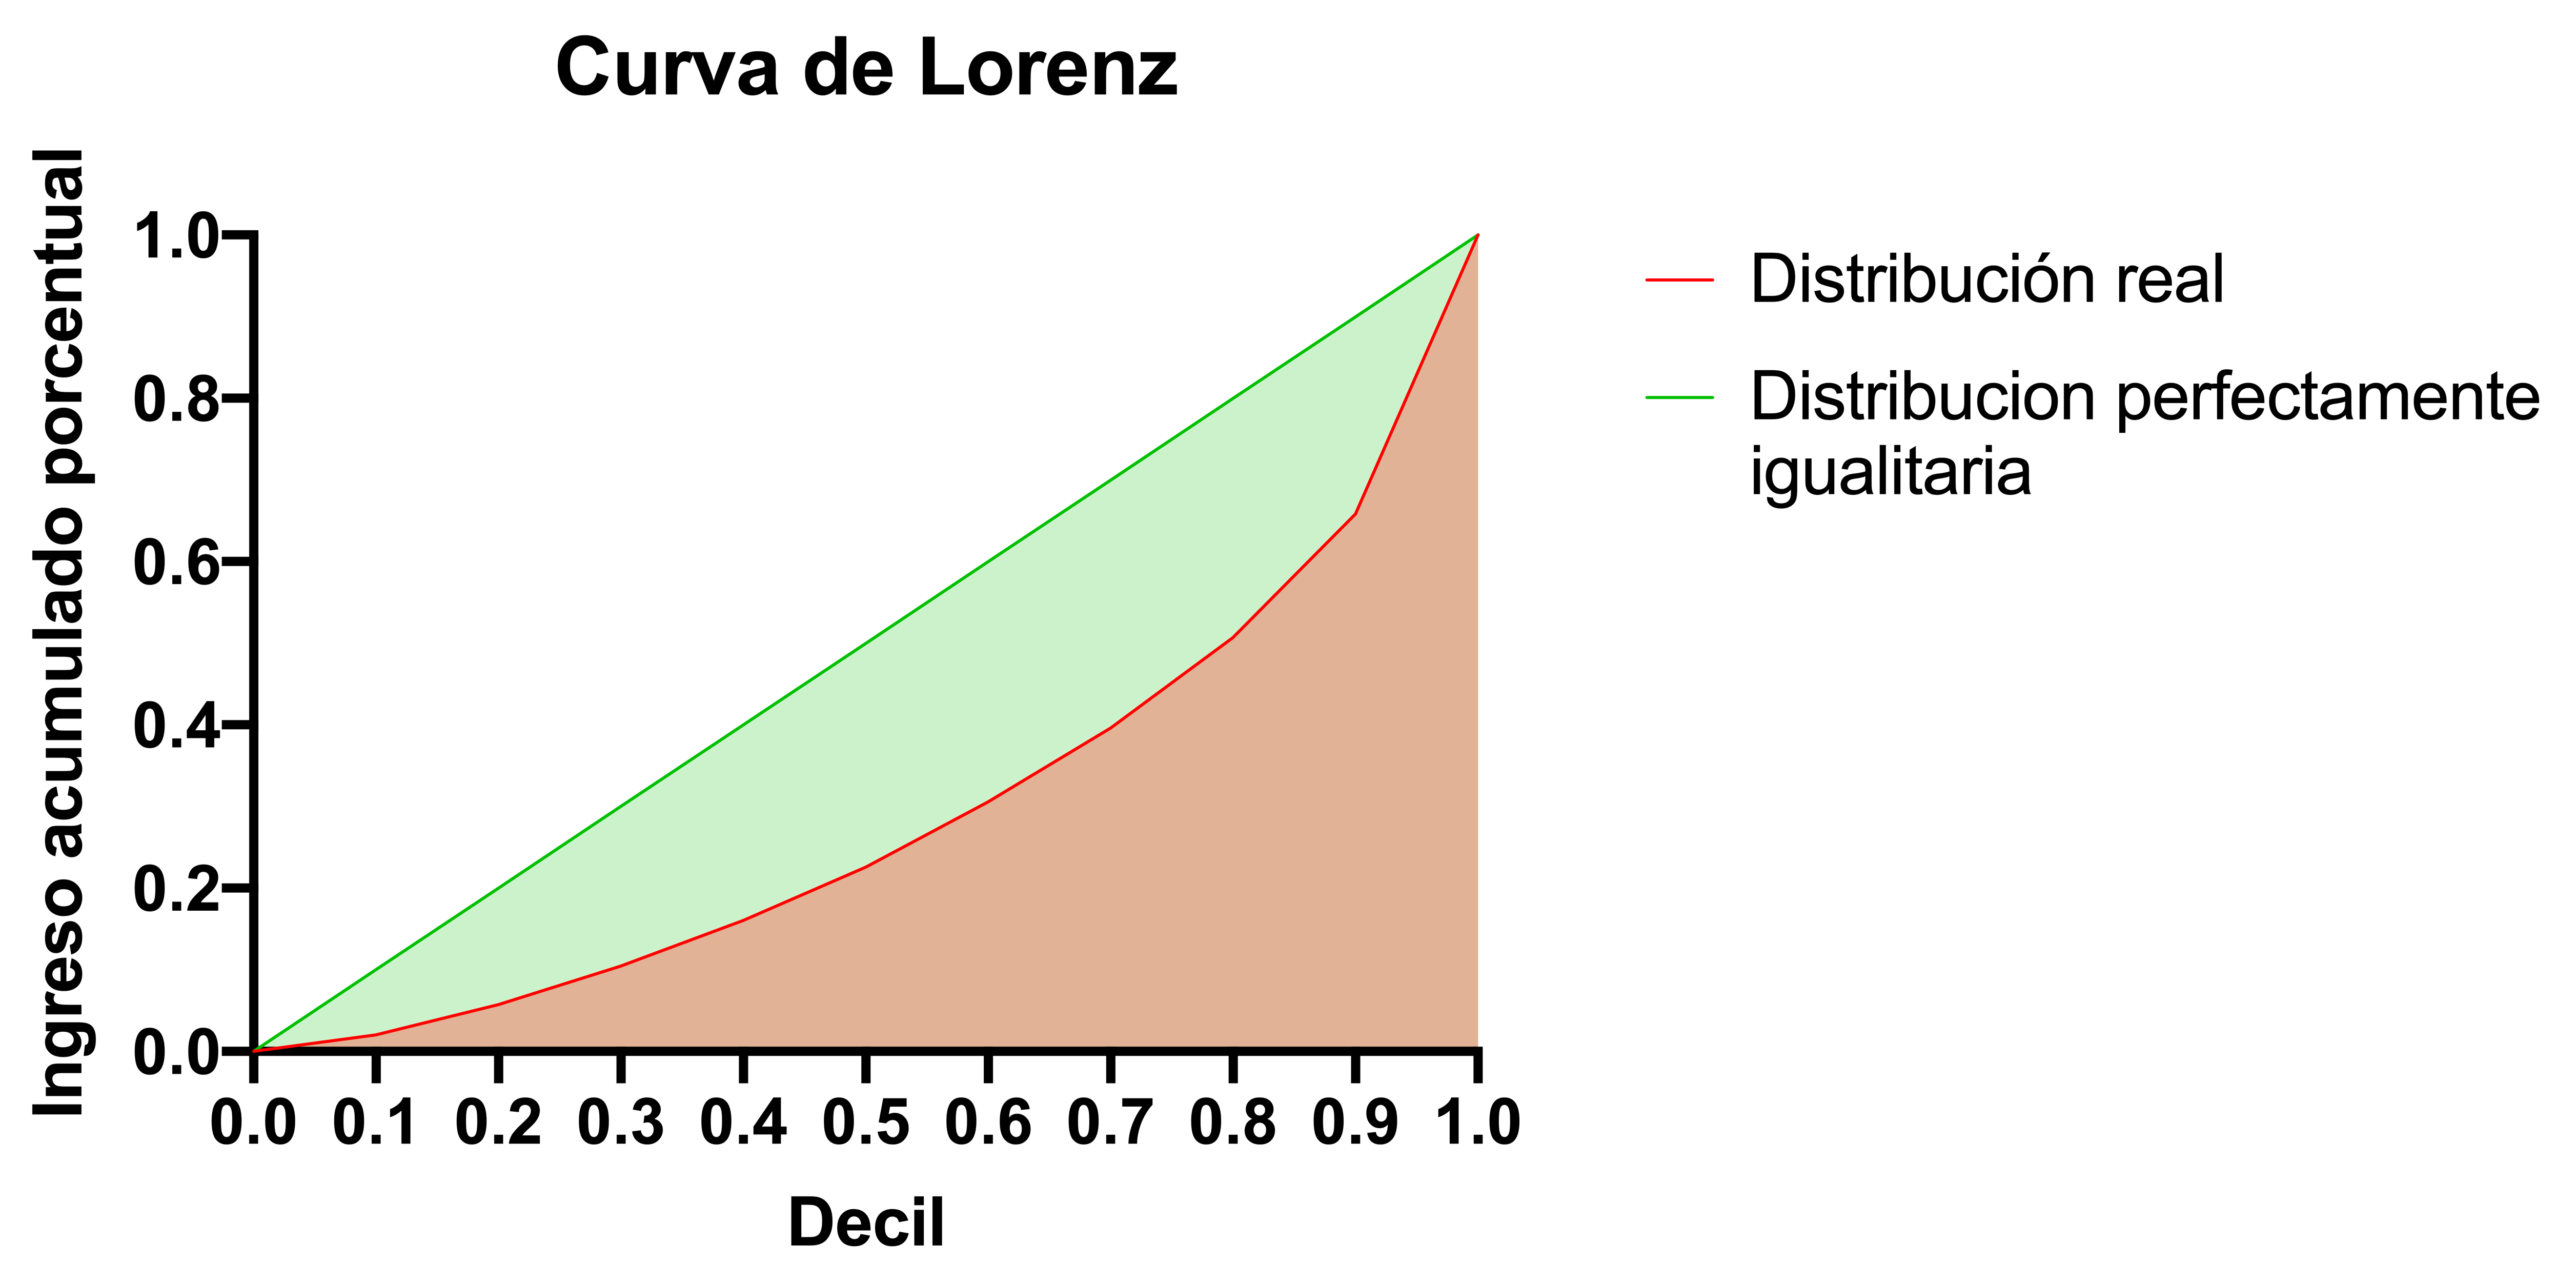
\includegraphics[width=0.84\textwidth]{Modulo_4/Curva_Lorenz_Final.png}
    \caption{Curva de Lorenz correspondiente a Chile, Casen 2017}
    \label{fig:lorenz_casen_2017}
\end{figure}

La figura \ref{fig:lorenz_casen_2017} muestra la curva de Lorenz correspondiente a Chile según la encuesta Casen 2017. En esta se puede observar en el eje vertical el \textit{Ingreso acumulado porcentual} y en el eje horizontal el \textit{Decil correspondiente} donde $0.1$ corresponde al decil 1, y así sucesivamente. \hfill \break


El índice de Gini se puede calcular a partir de las áreas bajo la curva del gráfico. Dividiendo el área entre la curva de la DPI y la distribución real, y sobre el área total. 
\[G = \frac{A_{DPI} - A_{DR}}{A_{total}}\]


En el caso de la figura \ref{fig:lorenz_casen_2017}, correspondería a dividir el área verde sobre la suma de las áreas verde y naranja. 
\newpage
\section{Criterios de asignación}

\econ{https://www.core-econ.org/the-economy/book/es/text/05.html}{5}

\subsection{Criterios de asignación}
Se entiende una asignación como el resultado de un determinado proceso económico.

\subsection{Eficiencia de Pareto}
Sean $A$ y $B$ asignaciones, la eficiencia de pareto establece que:
\hfill \break
\hfill \break
\textit{La asignación $A$ prevalece sobre la asignación $B$, si al menos una de las partes estaría mejor con $A$ que con $B$, y nadie estaría peor. En este caso $A$ domina a $B$ en términos de Pareto.}
\hfill \break


Una asignación que no está dominada en términos de Pareto se denomina \textbf{Pareto-eficiente.}


Este criterio es lo que en matemáticas se conoce como un orden parcial. Es decir, permite ordenar algunas asignaciones, pero no todas (esto sería un orden completo).

\subsubsection{Comentarios sobre la eficiencia de Pareto}
El criterio de la eficiencia de Pareto es uno de los conceptos más relevantes en economía. 


Dado un problema determinado, pueden existir muchas asignaciones que son pareto-eficientes. Pero sin un criterio adicional, no podemos decir cual de ellas es preferible.


Que una asignación sea eficiente de Pareto, no significa que estemos de acuerdo con ella. De hecho, si se le entregara todo el ingreso a una persona en la sociedad y dejamos a todo el resto sin nada, esa asignación es Pareto-Eficiente, pero probablemente no estemos de acuerdo en que sea una buena asignación económica.


Además, en muchas ocasiones, existe más de una asignación eficiente en términos de Pareto.

\subsection{Asignaciones}
Existen distintos casos posibles, y según este la manera de calcular asignación óptima varía.


\href{https://www.youtube.com/watch?v=jWcbHlTCPnQ}{Video EOL}
\begin{enumerate}[label=\Roman*.]
    \item \textbf{La persona genera el bien por si misma} \textit{(\href{https://youtu.be/jWcbHlTCPnQ?t=64}{Min 1:04})}, aquí $TMS = TMT$ es la condición de asignación óptima. 
    
    \item \textbf{Coerción} \textit{(\href{https://youtu.be/jWcbHlTCPnQ?t=181}{Min 3:01})}: alguien obliga a la persona a trabajar y se queda con los excedentes luego de darle lo mínimo que necesita la persona para subsistir (esclavitud). Existe una \textit{restricción de supervivencia biológica (RSB)}.
    
    El coerzor escogerá el punto donde la distancia entre la frontera del conjunto factible y la curva de RSB sea mayor.\\
    
    $TMB = TMT$ es la asignación óptima. (TMB es la tasa relacionada con RSB)
    
    \item \textbf{Propiedad privada} \textit{(\href{https://youtu.be/jWcbHlTCPnQ?t=333}{Min 5:33})}: La otra persona tiene todo el poder de negociación pero la primera persona solo trabajará si obtiene ganancias. \\
    
    Alguien externo (e.g. Estado o familia) ofrece una producción de sobrevivencia.\\
    
    Existe una curva de indiferencia de la primera persona. Se busca maximizar la distancia entre esa curva y la frontera factible.\\
    
    $TMT = TMS$ es la condición de optimalidad.
    
    \item \textbf{Negociación colectiva} \textit{(\href{https://youtu.be/jWcbHlTCPnQ?t=510}{Min 8:30})}: La primera persona busca parte del excedente.\\
    
    Una \hyperlink{institucion}{institución} externa (e.g. Estado) establece una curva de indiferencia nueva que ha de cumplirse, no necesariamente es Pareto-eficiente.\\
    
    A la persona se le puede ofrecer una nueva curva de indiferencia que le deje con igual igual utilidad (y que cumpla lo propuesto por el Estado) o que deje a ambas partes mejor.\\
    
    $TMT = TMS$ es la condición de optimalidad.
\end{enumerate}

\subsection{Desigualdad (criterios)}
Existen distintos tipos de medida a la hora de medir desigualdad, entre estas están

\begin{itemize}
    \item \textbf{Desigualdad absoluta}: es la resta de ingresos. Posee un problema que es que posee unidades dimensionales de ingreso lo cual hace difícil comparar entre lugares que no poseen las mismas unidades monetarias. Además aumenta cuando el país crece, aunque ambos ingresos crezcan a la misma \textit{tasa}. $\quad DA = Y_R - Y_P$
    
    \item \textbf{Desigualdad relativa}: es la división entre los ingresos. Es adimensional y no aumenta trivialmente cuando el país crece. $\quad DR = Y_R/Y_P$
\end{itemize}

Por esto es preferible hacer uso de la desigualdad relativa.

\subsubsection{Razones o \textit{ratios} de desigualdad}
Es la medida más sencilla de desigualdad, es la razón entre los ingresos de los sectores más ricos y pobres de la sociedad.

\begin{itemize}
    \item Razones entre quintiles
    \item Razones entre deciles
\end{itemize}

\subsubsection{Razón o índice de Palma}
Es un refinamiento de los \textit{ratios}, este índice considera que hay 3 grupos en la sociedad
\begin{enumerate}[label=\arabic*)]
    \item Los ricos (decil 10)
    \item Clase media (Decil 5 a 9)
    \item Los pobres (Decil 1 a 4)
\end{enumerate}

Se sustenta con la observación empírica: la clase media tiende a capturar la mitad del ingreso. 

\[\text{Razón de palma} = \frac{D_{10}}{D_1+D_2+D_3+D_4}\]

\subsubsection{Coeficiente o índice de Gini}
Es la medida más usada de desigualdad, representa que tanto se aleja una distribución real de una distribución totalmente igualitaria. Su valor varía entre 0 y 1, siendo mínima la desigualdad en 0 y máxima en 1. Posee dos formas:

\begin{enumerate}[label=\roman*.]
    \item \textbf{Forma general}: promedio de las diferencias de ingreso entre todos los individuos en una economía. Se calcula como \newline
    \[G = \frac{\sum_i\sum_j\abs{y_i-y_j}}{2\sum_{ij}y_i}\]
    
    \item \textbf{Forma de Sen}: suma ponderada de ingresos. (más usada)
    \newline
    \[G = \frac{2}{n}\frac{\sum_i^n i y_i}{\sum_i^n y_i} - \frac{n+1}{n}\]
\end{enumerate}


Donde $y_i$ son los ingresos correspondientes a $i$, e $i$ pueden ser deciles, quintiles, personas, etc. de las que hay una cantidad $n$.
\\

La interpretación más usual del coeficiente de Gini es a partir de la curva de Lorenz.
\subsubsection{Curva de Lorenz}
Muestra los ingresos acumulados desde los individuos más pobres a los más ricos de la sociedad. Comparándolos con la curva correspondiente a una distribución perfectamente igualitaria (DPI).

\begin{figure}[H]
    \centering
    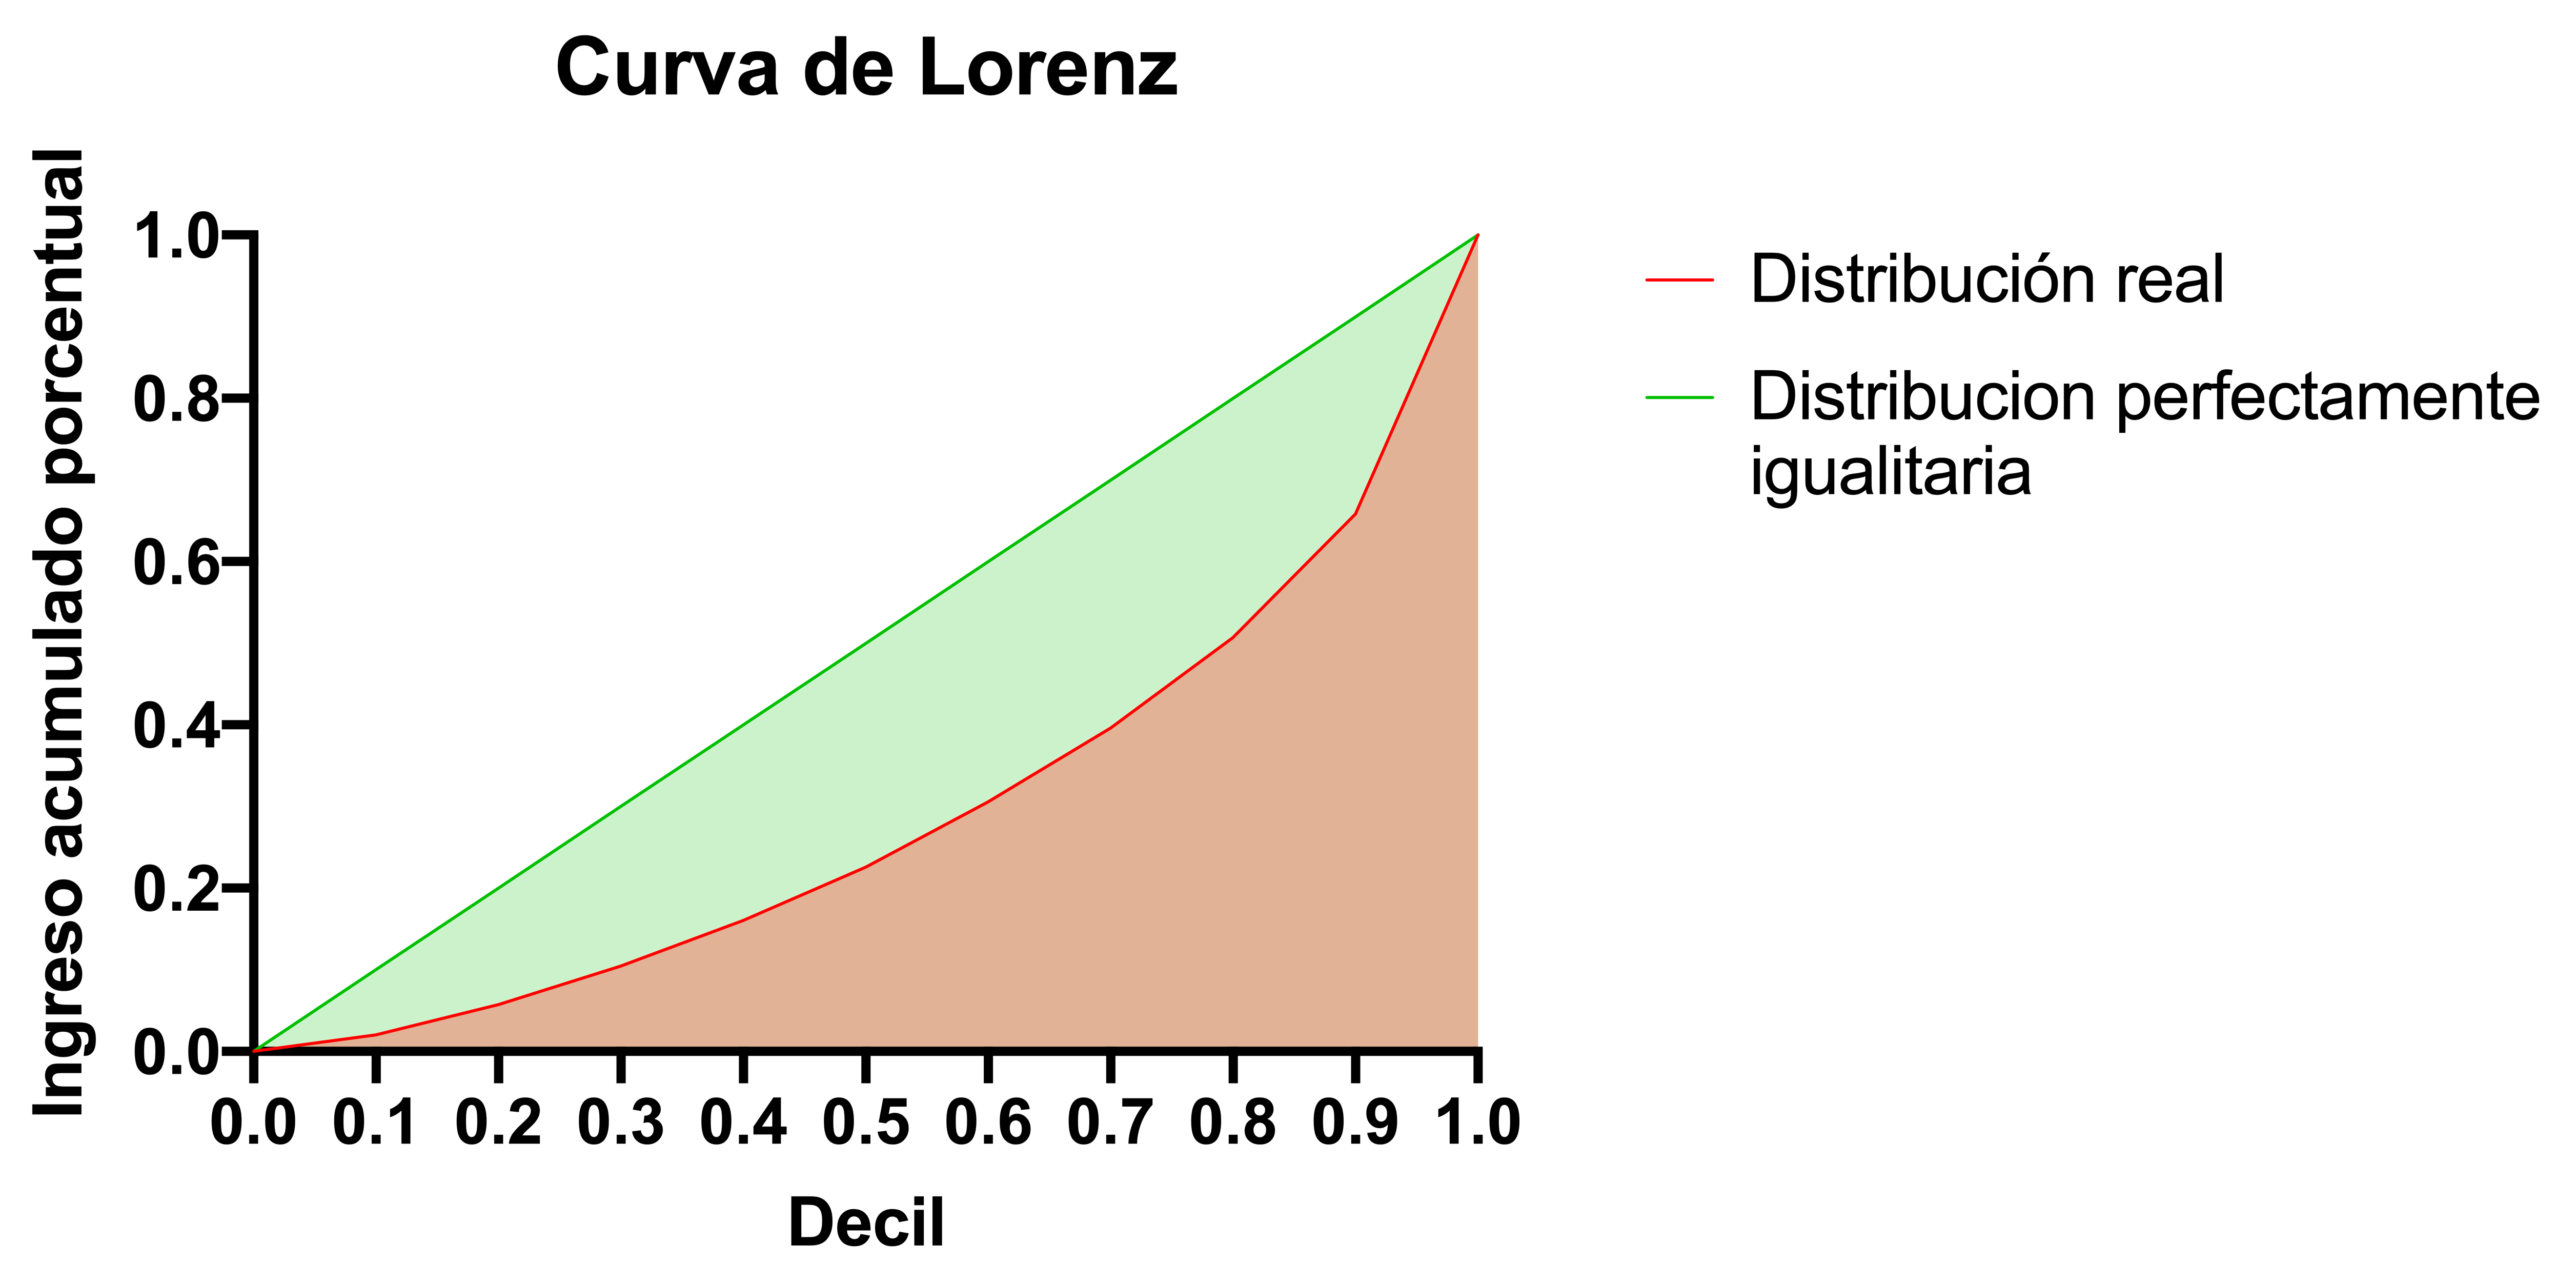
\includegraphics[width=0.84\textwidth]{Modulo_4/Curva_Lorenz_Final.png}
    \caption{Curva de Lorenz correspondiente a Chile, Casen 2017}
    \label{fig:lorenz_casen_2017}
\end{figure}

La figura \ref{fig:lorenz_casen_2017} muestra la curva de Lorenz correspondiente a Chile según la encuesta Casen 2017. En esta se puede observar en el eje vertical el \textit{Ingreso acumulado porcentual} y en el eje horizontal el \textit{Decil correspondiente} donde $0.1$ corresponde al decil 1, y así sucesivamente. \hfill \break


El índice de Gini se puede calcular a partir de las áreas bajo la curva del gráfico. Dividiendo el área entre la curva de la DPI y la distribución real, y sobre el área total. 
\[G = \frac{A_{DPI} - A_{DR}}{A_{total}}\]


En el caso de la figura \ref{fig:lorenz_casen_2017}, correspondería a dividir el área verde sobre la suma de las áreas verde y naranja. 
\newpage
\section{Criterios de asignación}

\econ{https://www.core-econ.org/the-economy/book/es/text/05.html}{5}

\subsection{Criterios de asignación}
Se entiende una asignación como el resultado de un determinado proceso económico.

\subsection{Eficiencia de Pareto}
Sean $A$ y $B$ asignaciones, la eficiencia de pareto establece que:
\hfill \break
\hfill \break
\textit{La asignación $A$ prevalece sobre la asignación $B$, si al menos una de las partes estaría mejor con $A$ que con $B$, y nadie estaría peor. En este caso $A$ domina a $B$ en términos de Pareto.}
\hfill \break


Una asignación que no está dominada en términos de Pareto se denomina \textbf{Pareto-eficiente.}


Este criterio es lo que en matemáticas se conoce como un orden parcial. Es decir, permite ordenar algunas asignaciones, pero no todas (esto sería un orden completo).

\subsubsection{Comentarios sobre la eficiencia de Pareto}
El criterio de la eficiencia de Pareto es uno de los conceptos más relevantes en economía. 


Dado un problema determinado, pueden existir muchas asignaciones que son pareto-eficientes. Pero sin un criterio adicional, no podemos decir cual de ellas es preferible.


Que una asignación sea eficiente de Pareto, no significa que estemos de acuerdo con ella. De hecho, si se le entregara todo el ingreso a una persona en la sociedad y dejamos a todo el resto sin nada, esa asignación es Pareto-Eficiente, pero probablemente no estemos de acuerdo en que sea una buena asignación económica.


Además, en muchas ocasiones, existe más de una asignación eficiente en términos de Pareto.

\subsection{Asignaciones}
Existen distintos casos posibles, y según este la manera de calcular asignación óptima varía.


\href{https://www.youtube.com/watch?v=jWcbHlTCPnQ}{Video EOL}
\begin{enumerate}[label=\Roman*.]
    \item \textbf{La persona genera el bien por si misma} \textit{(\href{https://youtu.be/jWcbHlTCPnQ?t=64}{Min 1:04})}, aquí $TMS = TMT$ es la condición de asignación óptima. 
    
    \item \textbf{Coerción} \textit{(\href{https://youtu.be/jWcbHlTCPnQ?t=181}{Min 3:01})}: alguien obliga a la persona a trabajar y se queda con los excedentes luego de darle lo mínimo que necesita la persona para subsistir (esclavitud). Existe una \textit{restricción de supervivencia biológica (RSB)}.
    
    El coerzor escogerá el punto donde la distancia entre la frontera del conjunto factible y la curva de RSB sea mayor.\\
    
    $TMB = TMT$ es la asignación óptima. (TMB es la tasa relacionada con RSB)
    
    \item \textbf{Propiedad privada} \textit{(\href{https://youtu.be/jWcbHlTCPnQ?t=333}{Min 5:33})}: La otra persona tiene todo el poder de negociación pero la primera persona solo trabajará si obtiene ganancias. \\
    
    Alguien externo (e.g. Estado o familia) ofrece una producción de sobrevivencia.\\
    
    Existe una curva de indiferencia de la primera persona. Se busca maximizar la distancia entre esa curva y la frontera factible.\\
    
    $TMT = TMS$ es la condición de optimalidad.
    
    \item \textbf{Negociación colectiva} \textit{(\href{https://youtu.be/jWcbHlTCPnQ?t=510}{Min 8:30})}: La primera persona busca parte del excedente.\\
    
    Una \hyperlink{institucion}{institución} externa (e.g. Estado) establece una curva de indiferencia nueva que ha de cumplirse, no necesariamente es Pareto-eficiente.\\
    
    A la persona se le puede ofrecer una nueva curva de indiferencia que le deje con igual igual utilidad (y que cumpla lo propuesto por el Estado) o que deje a ambas partes mejor.\\
    
    $TMT = TMS$ es la condición de optimalidad.
\end{enumerate}

\subsection{Desigualdad (criterios)}
Existen distintos tipos de medida a la hora de medir desigualdad, entre estas están

\begin{itemize}
    \item \textbf{Desigualdad absoluta}: es la resta de ingresos. Posee un problema que es que posee unidades dimensionales de ingreso lo cual hace difícil comparar entre lugares que no poseen las mismas unidades monetarias. Además aumenta cuando el país crece, aunque ambos ingresos crezcan a la misma \textit{tasa}. $\quad DA = Y_R - Y_P$
    
    \item \textbf{Desigualdad relativa}: es la división entre los ingresos. Es adimensional y no aumenta trivialmente cuando el país crece. $\quad DR = Y_R/Y_P$
\end{itemize}

Por esto es preferible hacer uso de la desigualdad relativa.

\subsubsection{Razones o \textit{ratios} de desigualdad}
Es la medida más sencilla de desigualdad, es la razón entre los ingresos de los sectores más ricos y pobres de la sociedad.

\begin{itemize}
    \item Razones entre quintiles
    \item Razones entre deciles
\end{itemize}

\subsubsection{Razón o índice de Palma}
Es un refinamiento de los \textit{ratios}, este índice considera que hay 3 grupos en la sociedad
\begin{enumerate}[label=\arabic*)]
    \item Los ricos (decil 10)
    \item Clase media (Decil 5 a 9)
    \item Los pobres (Decil 1 a 4)
\end{enumerate}

Se sustenta con la observación empírica: la clase media tiende a capturar la mitad del ingreso. 

\[\text{Razón de palma} = \frac{D_{10}}{D_1+D_2+D_3+D_4}\]

\subsubsection{Coeficiente o índice de Gini}
Es la medida más usada de desigualdad, representa que tanto se aleja una distribución real de una distribución totalmente igualitaria. Su valor varía entre 0 y 1, siendo mínima la desigualdad en 0 y máxima en 1. Posee dos formas:

\begin{enumerate}[label=\roman*.]
    \item \textbf{Forma general}: promedio de las diferencias de ingreso entre todos los individuos en una economía. Se calcula como \newline
    \[G = \frac{\sum_i\sum_j\abs{y_i-y_j}}{2\sum_{ij}y_i}\]
    
    \item \textbf{Forma de Sen}: suma ponderada de ingresos. (más usada)
    \newline
    \[G = \frac{2}{n}\frac{\sum_i^n i y_i}{\sum_i^n y_i} - \frac{n+1}{n}\]
\end{enumerate}


Donde $y_i$ son los ingresos correspondientes a $i$, e $i$ pueden ser deciles, quintiles, personas, etc. de las que hay una cantidad $n$.
\\

La interpretación más usual del coeficiente de Gini es a partir de la curva de Lorenz.
\subsubsection{Curva de Lorenz}
Muestra los ingresos acumulados desde los individuos más pobres a los más ricos de la sociedad. Comparándolos con la curva correspondiente a una distribución perfectamente igualitaria (DPI).

\begin{figure}[H]
    \centering
    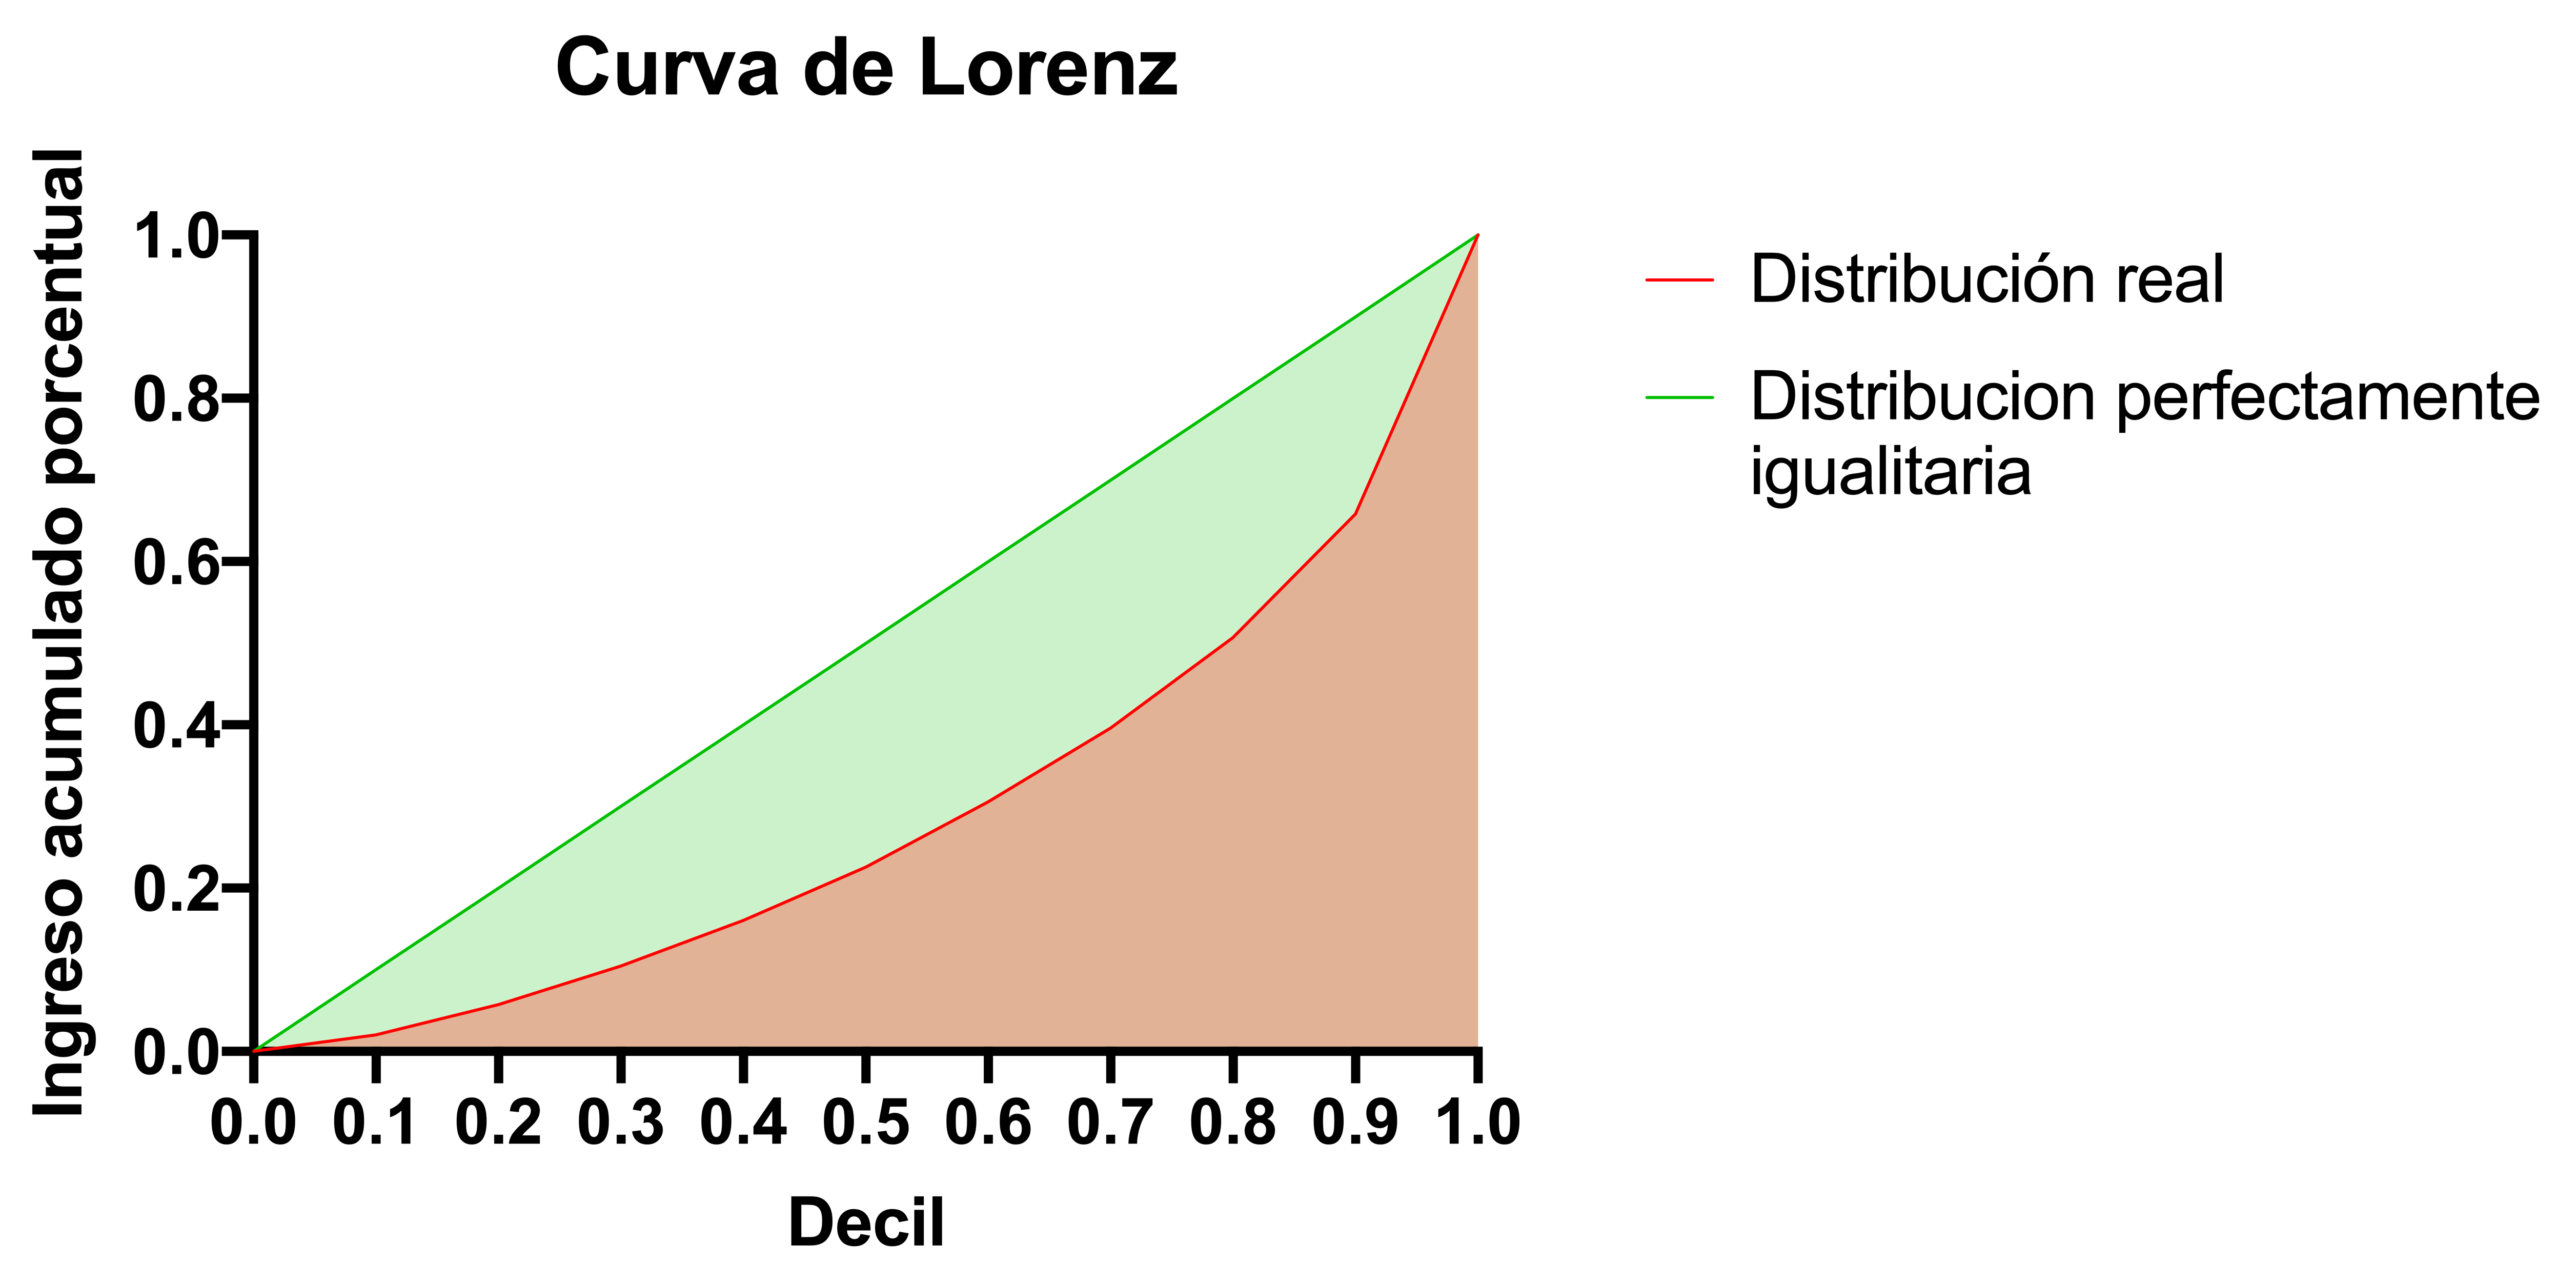
\includegraphics[width=0.84\textwidth]{Modulo_4/Curva_Lorenz_Final.png}
    \caption{Curva de Lorenz correspondiente a Chile, Casen 2017}
    \label{fig:lorenz_casen_2017}
\end{figure}

La figura \ref{fig:lorenz_casen_2017} muestra la curva de Lorenz correspondiente a Chile según la encuesta Casen 2017. En esta se puede observar en el eje vertical el \textit{Ingreso acumulado porcentual} y en el eje horizontal el \textit{Decil correspondiente} donde $0.1$ corresponde al decil 1, y así sucesivamente. \hfill \break


El índice de Gini se puede calcular a partir de las áreas bajo la curva del gráfico. Dividiendo el área entre la curva de la DPI y la distribución real, y sobre el área total. 
\[G = \frac{A_{DPI} - A_{DR}}{A_{total}}\]


En el caso de la figura \ref{fig:lorenz_casen_2017}, correspondería a dividir el área verde sobre la suma de las áreas verde y naranja. 
\newpage
\section{Criterios de asignación}

\econ{https://www.core-econ.org/the-economy/book/es/text/05.html}{5}

\subsection{Criterios de asignación}
Se entiende una asignación como el resultado de un determinado proceso económico.

\subsection{Eficiencia de Pareto}
Sean $A$ y $B$ asignaciones, la eficiencia de pareto establece que:
\hfill \break
\hfill \break
\textit{La asignación $A$ prevalece sobre la asignación $B$, si al menos una de las partes estaría mejor con $A$ que con $B$, y nadie estaría peor. En este caso $A$ domina a $B$ en términos de Pareto.}
\hfill \break


Una asignación que no está dominada en términos de Pareto se denomina \textbf{Pareto-eficiente.}


Este criterio es lo que en matemáticas se conoce como un orden parcial. Es decir, permite ordenar algunas asignaciones, pero no todas (esto sería un orden completo).

\subsubsection{Comentarios sobre la eficiencia de Pareto}
El criterio de la eficiencia de Pareto es uno de los conceptos más relevantes en economía. 


Dado un problema determinado, pueden existir muchas asignaciones que son pareto-eficientes. Pero sin un criterio adicional, no podemos decir cual de ellas es preferible.


Que una asignación sea eficiente de Pareto, no significa que estemos de acuerdo con ella. De hecho, si se le entregara todo el ingreso a una persona en la sociedad y dejamos a todo el resto sin nada, esa asignación es Pareto-Eficiente, pero probablemente no estemos de acuerdo en que sea una buena asignación económica.


Además, en muchas ocasiones, existe más de una asignación eficiente en términos de Pareto.

\subsection{Asignaciones}
Existen distintos casos posibles, y según este la manera de calcular asignación óptima varía.


\href{https://www.youtube.com/watch?v=jWcbHlTCPnQ}{Video EOL}
\begin{enumerate}[label=\Roman*.]
    \item \textbf{La persona genera el bien por si misma} \textit{(\href{https://youtu.be/jWcbHlTCPnQ?t=64}{Min 1:04})}, aquí $TMS = TMT$ es la condición de asignación óptima. 
    
    \item \textbf{Coerción} \textit{(\href{https://youtu.be/jWcbHlTCPnQ?t=181}{Min 3:01})}: alguien obliga a la persona a trabajar y se queda con los excedentes luego de darle lo mínimo que necesita la persona para subsistir (esclavitud). Existe una \textit{restricción de supervivencia biológica (RSB)}.
    
    El coerzor escogerá el punto donde la distancia entre la frontera del conjunto factible y la curva de RSB sea mayor.\\
    
    $TMB = TMT$ es la asignación óptima. (TMB es la tasa relacionada con RSB)
    
    \item \textbf{Propiedad privada} \textit{(\href{https://youtu.be/jWcbHlTCPnQ?t=333}{Min 5:33})}: La otra persona tiene todo el poder de negociación pero la primera persona solo trabajará si obtiene ganancias. \\
    
    Alguien externo (e.g. Estado o familia) ofrece una producción de sobrevivencia.\\
    
    Existe una curva de indiferencia de la primera persona. Se busca maximizar la distancia entre esa curva y la frontera factible.\\
    
    $TMT = TMS$ es la condición de optimalidad.
    
    \item \textbf{Negociación colectiva} \textit{(\href{https://youtu.be/jWcbHlTCPnQ?t=510}{Min 8:30})}: La primera persona busca parte del excedente.\\
    
    Una \hyperlink{institucion}{institución} externa (e.g. Estado) establece una curva de indiferencia nueva que ha de cumplirse, no necesariamente es Pareto-eficiente.\\
    
    A la persona se le puede ofrecer una nueva curva de indiferencia que le deje con igual igual utilidad (y que cumpla lo propuesto por el Estado) o que deje a ambas partes mejor.\\
    
    $TMT = TMS$ es la condición de optimalidad.
\end{enumerate}

\subsection{Desigualdad (criterios)}
Existen distintos tipos de medida a la hora de medir desigualdad, entre estas están

\begin{itemize}
    \item \textbf{Desigualdad absoluta}: es la resta de ingresos. Posee un problema que es que posee unidades dimensionales de ingreso lo cual hace difícil comparar entre lugares que no poseen las mismas unidades monetarias. Además aumenta cuando el país crece, aunque ambos ingresos crezcan a la misma \textit{tasa}. $\quad DA = Y_R - Y_P$
    
    \item \textbf{Desigualdad relativa}: es la división entre los ingresos. Es adimensional y no aumenta trivialmente cuando el país crece. $\quad DR = Y_R/Y_P$
\end{itemize}

Por esto es preferible hacer uso de la desigualdad relativa.

\subsubsection{Razones o \textit{ratios} de desigualdad}
Es la medida más sencilla de desigualdad, es la razón entre los ingresos de los sectores más ricos y pobres de la sociedad.

\begin{itemize}
    \item Razones entre quintiles
    \item Razones entre deciles
\end{itemize}

\subsubsection{Razón o índice de Palma}
Es un refinamiento de los \textit{ratios}, este índice considera que hay 3 grupos en la sociedad
\begin{enumerate}[label=\arabic*)]
    \item Los ricos (decil 10)
    \item Clase media (Decil 5 a 9)
    \item Los pobres (Decil 1 a 4)
\end{enumerate}

Se sustenta con la observación empírica: la clase media tiende a capturar la mitad del ingreso. 

\[\text{Razón de palma} = \frac{D_{10}}{D_1+D_2+D_3+D_4}\]

\subsubsection{Coeficiente o índice de Gini}
Es la medida más usada de desigualdad, representa que tanto se aleja una distribución real de una distribución totalmente igualitaria. Su valor varía entre 0 y 1, siendo mínima la desigualdad en 0 y máxima en 1. Posee dos formas:

\begin{enumerate}[label=\roman*.]
    \item \textbf{Forma general}: promedio de las diferencias de ingreso entre todos los individuos en una economía. Se calcula como \newline
    \[G = \frac{\sum_i\sum_j\abs{y_i-y_j}}{2\sum_{ij}y_i}\]
    
    \item \textbf{Forma de Sen}: suma ponderada de ingresos. (más usada)
    \newline
    \[G = \frac{2}{n}\frac{\sum_i^n i y_i}{\sum_i^n y_i} - \frac{n+1}{n}\]
\end{enumerate}


Donde $y_i$ son los ingresos correspondientes a $i$, e $i$ pueden ser deciles, quintiles, personas, etc. de las que hay una cantidad $n$.
\\

La interpretación más usual del coeficiente de Gini es a partir de la curva de Lorenz.
\subsubsection{Curva de Lorenz}
Muestra los ingresos acumulados desde los individuos más pobres a los más ricos de la sociedad. Comparándolos con la curva correspondiente a una distribución perfectamente igualitaria (DPI).

\begin{figure}[H]
    \centering
    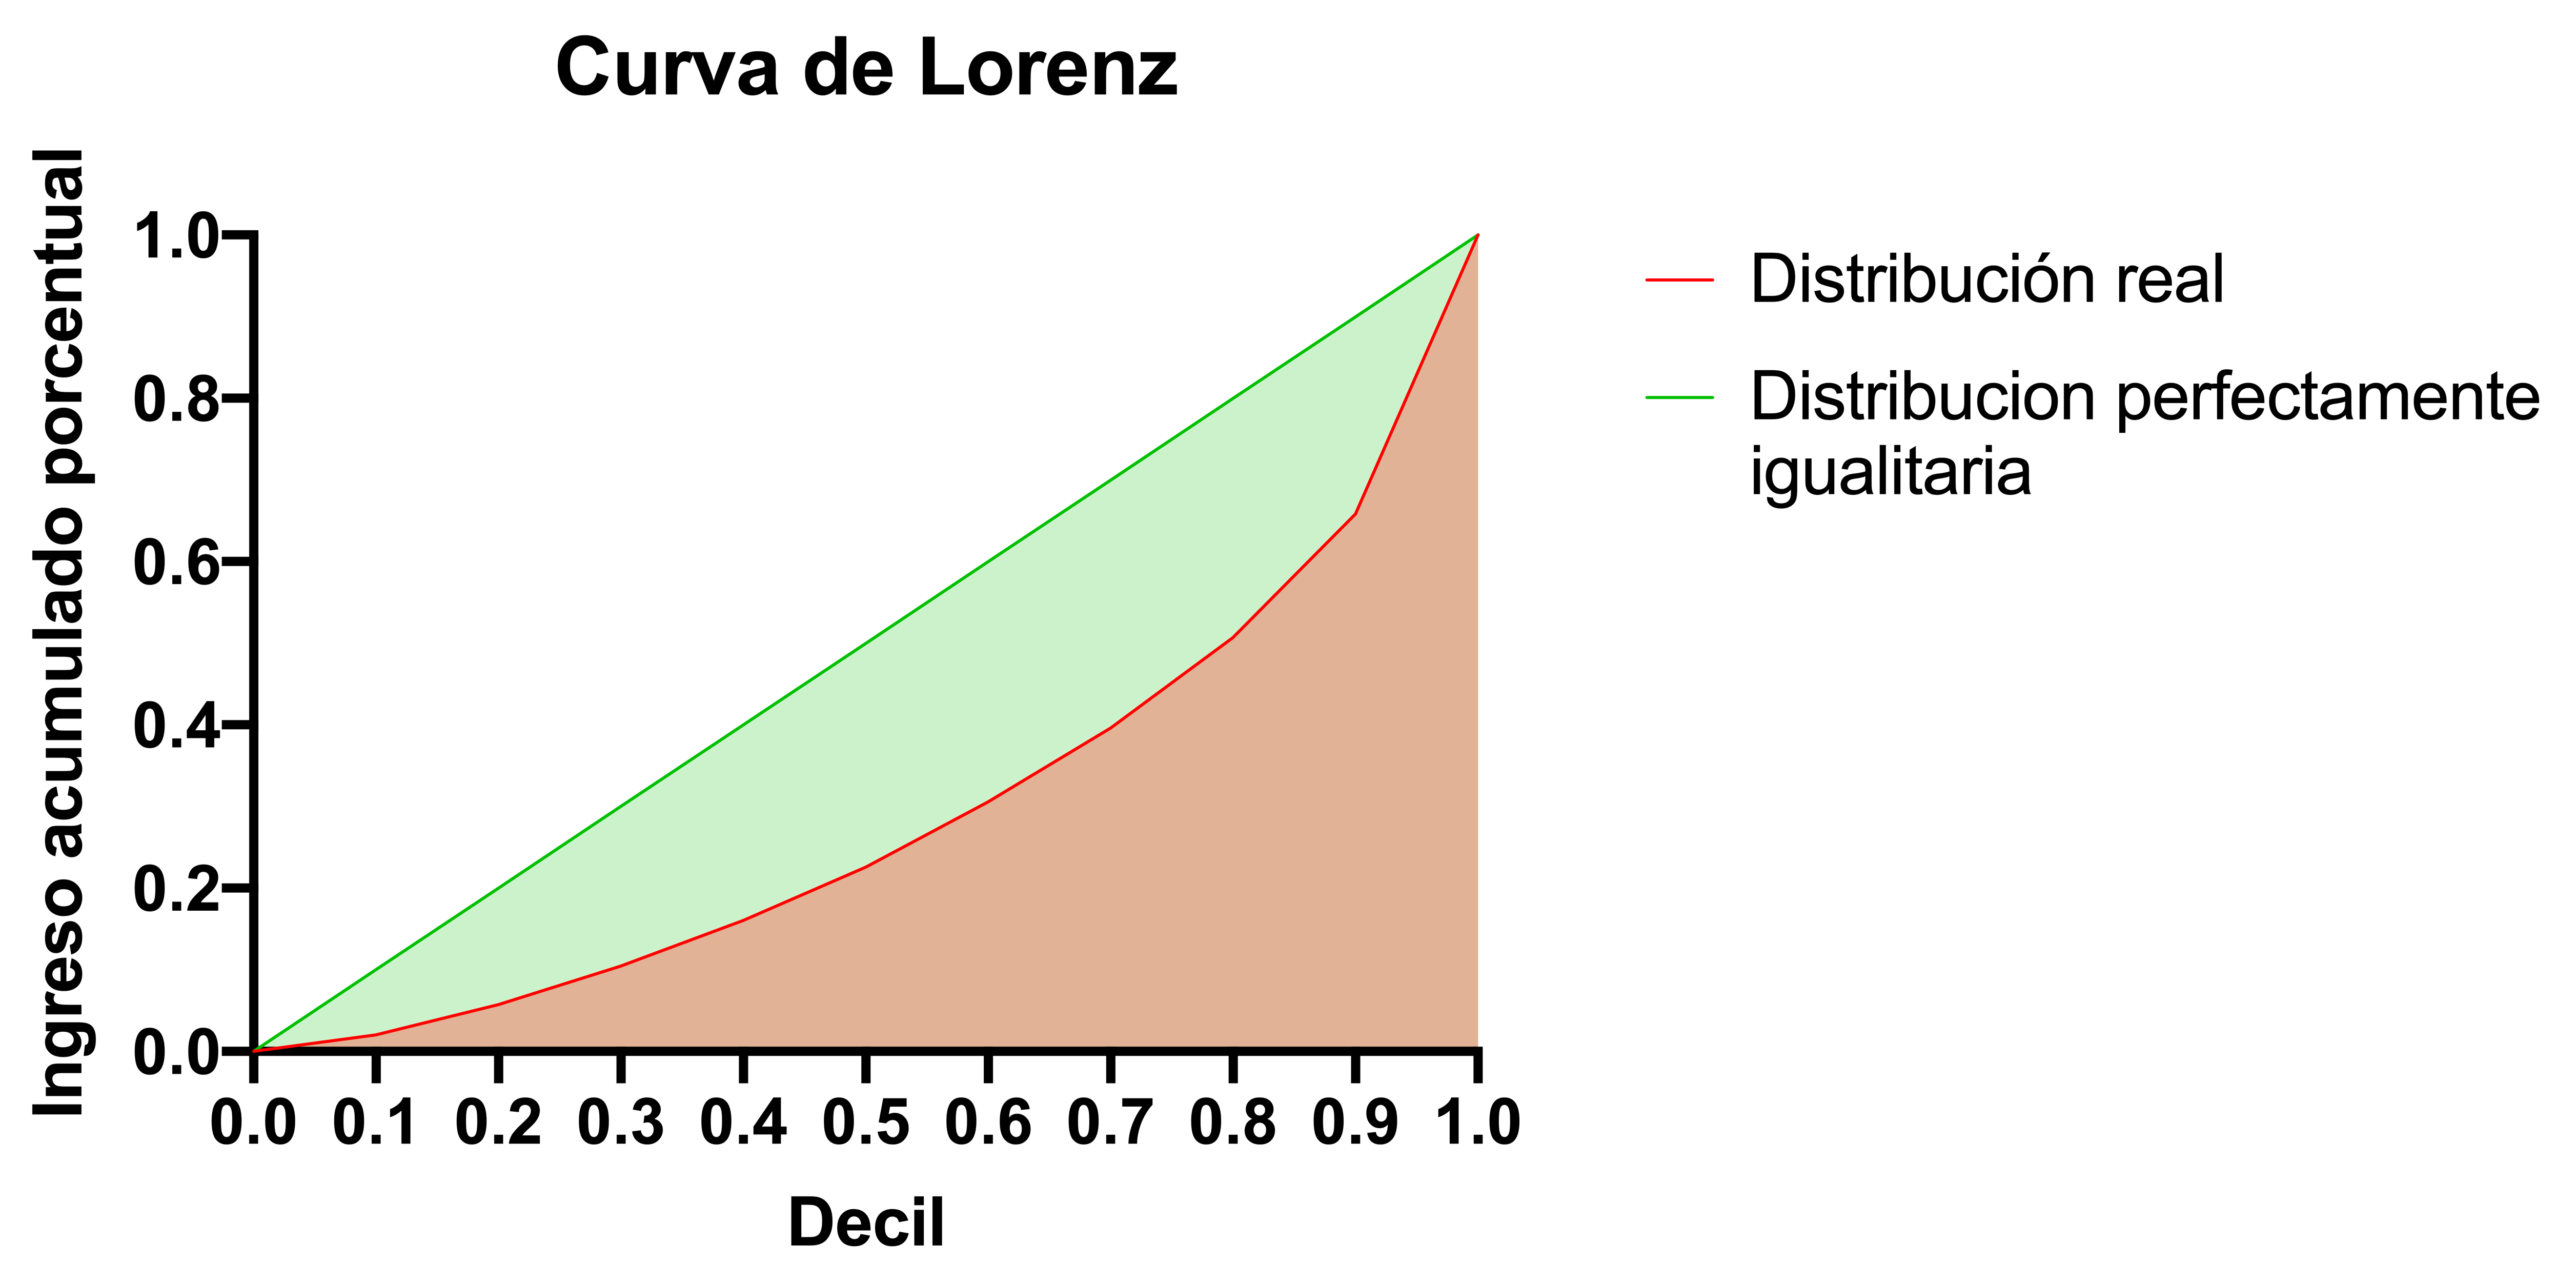
\includegraphics[width=0.84\textwidth]{Modulo_4/Curva_Lorenz_Final.png}
    \caption{Curva de Lorenz correspondiente a Chile, Casen 2017}
    \label{fig:lorenz_casen_2017}
\end{figure}

La figura \ref{fig:lorenz_casen_2017} muestra la curva de Lorenz correspondiente a Chile según la encuesta Casen 2017. En esta se puede observar en el eje vertical el \textit{Ingreso acumulado porcentual} y en el eje horizontal el \textit{Decil correspondiente} donde $0.1$ corresponde al decil 1, y así sucesivamente. \hfill \break


El índice de Gini se puede calcular a partir de las áreas bajo la curva del gráfico. Dividiendo el área entre la curva de la DPI y la distribución real, y sobre el área total. 
\[G = \frac{A_{DPI} - A_{DR}}{A_{total}}\]


En el caso de la figura \ref{fig:lorenz_casen_2017}, correspondería a dividir el área verde sobre la suma de las áreas verde y naranja. 
\newpage
\section{Criterios de asignación}

\econ{https://www.core-econ.org/the-economy/book/es/text/05.html}{5}

\subsection{Criterios de asignación}
Se entiende una asignación como el resultado de un determinado proceso económico.

\subsection{Eficiencia de Pareto}
Sean $A$ y $B$ asignaciones, la eficiencia de pareto establece que:
\hfill \break
\hfill \break
\textit{La asignación $A$ prevalece sobre la asignación $B$, si al menos una de las partes estaría mejor con $A$ que con $B$, y nadie estaría peor. En este caso $A$ domina a $B$ en términos de Pareto.}
\hfill \break


Una asignación que no está dominada en términos de Pareto se denomina \textbf{Pareto-eficiente.}


Este criterio es lo que en matemáticas se conoce como un orden parcial. Es decir, permite ordenar algunas asignaciones, pero no todas (esto sería un orden completo).

\subsubsection{Comentarios sobre la eficiencia de Pareto}
El criterio de la eficiencia de Pareto es uno de los conceptos más relevantes en economía. 


Dado un problema determinado, pueden existir muchas asignaciones que son pareto-eficientes. Pero sin un criterio adicional, no podemos decir cual de ellas es preferible.


Que una asignación sea eficiente de Pareto, no significa que estemos de acuerdo con ella. De hecho, si se le entregara todo el ingreso a una persona en la sociedad y dejamos a todo el resto sin nada, esa asignación es Pareto-Eficiente, pero probablemente no estemos de acuerdo en que sea una buena asignación económica.


Además, en muchas ocasiones, existe más de una asignación eficiente en términos de Pareto.

\subsection{Asignaciones}
Existen distintos casos posibles, y según este la manera de calcular asignación óptima varía.


\href{https://www.youtube.com/watch?v=jWcbHlTCPnQ}{Video EOL}
\begin{enumerate}[label=\Roman*.]
    \item \textbf{La persona genera el bien por si misma} \textit{(\href{https://youtu.be/jWcbHlTCPnQ?t=64}{Min 1:04})}, aquí $TMS = TMT$ es la condición de asignación óptima. 
    
    \item \textbf{Coerción} \textit{(\href{https://youtu.be/jWcbHlTCPnQ?t=181}{Min 3:01})}: alguien obliga a la persona a trabajar y se queda con los excedentes luego de darle lo mínimo que necesita la persona para subsistir (esclavitud). Existe una \textit{restricción de supervivencia biológica (RSB)}.
    
    El coerzor escogerá el punto donde la distancia entre la frontera del conjunto factible y la curva de RSB sea mayor.\\
    
    $TMB = TMT$ es la asignación óptima. (TMB es la tasa relacionada con RSB)
    
    \item \textbf{Propiedad privada} \textit{(\href{https://youtu.be/jWcbHlTCPnQ?t=333}{Min 5:33})}: La otra persona tiene todo el poder de negociación pero la primera persona solo trabajará si obtiene ganancias. \\
    
    Alguien externo (e.g. Estado o familia) ofrece una producción de sobrevivencia.\\
    
    Existe una curva de indiferencia de la primera persona. Se busca maximizar la distancia entre esa curva y la frontera factible.\\
    
    $TMT = TMS$ es la condición de optimalidad.
    
    \item \textbf{Negociación colectiva} \textit{(\href{https://youtu.be/jWcbHlTCPnQ?t=510}{Min 8:30})}: La primera persona busca parte del excedente.\\
    
    Una \hyperlink{institucion}{institución} externa (e.g. Estado) establece una curva de indiferencia nueva que ha de cumplirse, no necesariamente es Pareto-eficiente.\\
    
    A la persona se le puede ofrecer una nueva curva de indiferencia que le deje con igual igual utilidad (y que cumpla lo propuesto por el Estado) o que deje a ambas partes mejor.\\
    
    $TMT = TMS$ es la condición de optimalidad.
\end{enumerate}

\subsection{Desigualdad (criterios)}
Existen distintos tipos de medida a la hora de medir desigualdad, entre estas están

\begin{itemize}
    \item \textbf{Desigualdad absoluta}: es la resta de ingresos. Posee un problema que es que posee unidades dimensionales de ingreso lo cual hace difícil comparar entre lugares que no poseen las mismas unidades monetarias. Además aumenta cuando el país crece, aunque ambos ingresos crezcan a la misma \textit{tasa}. $\quad DA = Y_R - Y_P$
    
    \item \textbf{Desigualdad relativa}: es la división entre los ingresos. Es adimensional y no aumenta trivialmente cuando el país crece. $\quad DR = Y_R/Y_P$
\end{itemize}

Por esto es preferible hacer uso de la desigualdad relativa.

\subsubsection{Razones o \textit{ratios} de desigualdad}
Es la medida más sencilla de desigualdad, es la razón entre los ingresos de los sectores más ricos y pobres de la sociedad.

\begin{itemize}
    \item Razones entre quintiles
    \item Razones entre deciles
\end{itemize}

\subsubsection{Razón o índice de Palma}
Es un refinamiento de los \textit{ratios}, este índice considera que hay 3 grupos en la sociedad
\begin{enumerate}[label=\arabic*)]
    \item Los ricos (decil 10)
    \item Clase media (Decil 5 a 9)
    \item Los pobres (Decil 1 a 4)
\end{enumerate}

Se sustenta con la observación empírica: la clase media tiende a capturar la mitad del ingreso. 

\[\text{Razón de palma} = \frac{D_{10}}{D_1+D_2+D_3+D_4}\]

\subsubsection{Coeficiente o índice de Gini}
Es la medida más usada de desigualdad, representa que tanto se aleja una distribución real de una distribución totalmente igualitaria. Su valor varía entre 0 y 1, siendo mínima la desigualdad en 0 y máxima en 1. Posee dos formas:

\begin{enumerate}[label=\roman*.]
    \item \textbf{Forma general}: promedio de las diferencias de ingreso entre todos los individuos en una economía. Se calcula como \newline
    \[G = \frac{\sum_i\sum_j\abs{y_i-y_j}}{2\sum_{ij}y_i}\]
    
    \item \textbf{Forma de Sen}: suma ponderada de ingresos. (más usada)
    \newline
    \[G = \frac{2}{n}\frac{\sum_i^n i y_i}{\sum_i^n y_i} - \frac{n+1}{n}\]
\end{enumerate}


Donde $y_i$ son los ingresos correspondientes a $i$, e $i$ pueden ser deciles, quintiles, personas, etc. de las que hay una cantidad $n$.
\\

La interpretación más usual del coeficiente de Gini es a partir de la curva de Lorenz.
\subsubsection{Curva de Lorenz}
Muestra los ingresos acumulados desde los individuos más pobres a los más ricos de la sociedad. Comparándolos con la curva correspondiente a una distribución perfectamente igualitaria (DPI).

\begin{figure}[H]
    \centering
    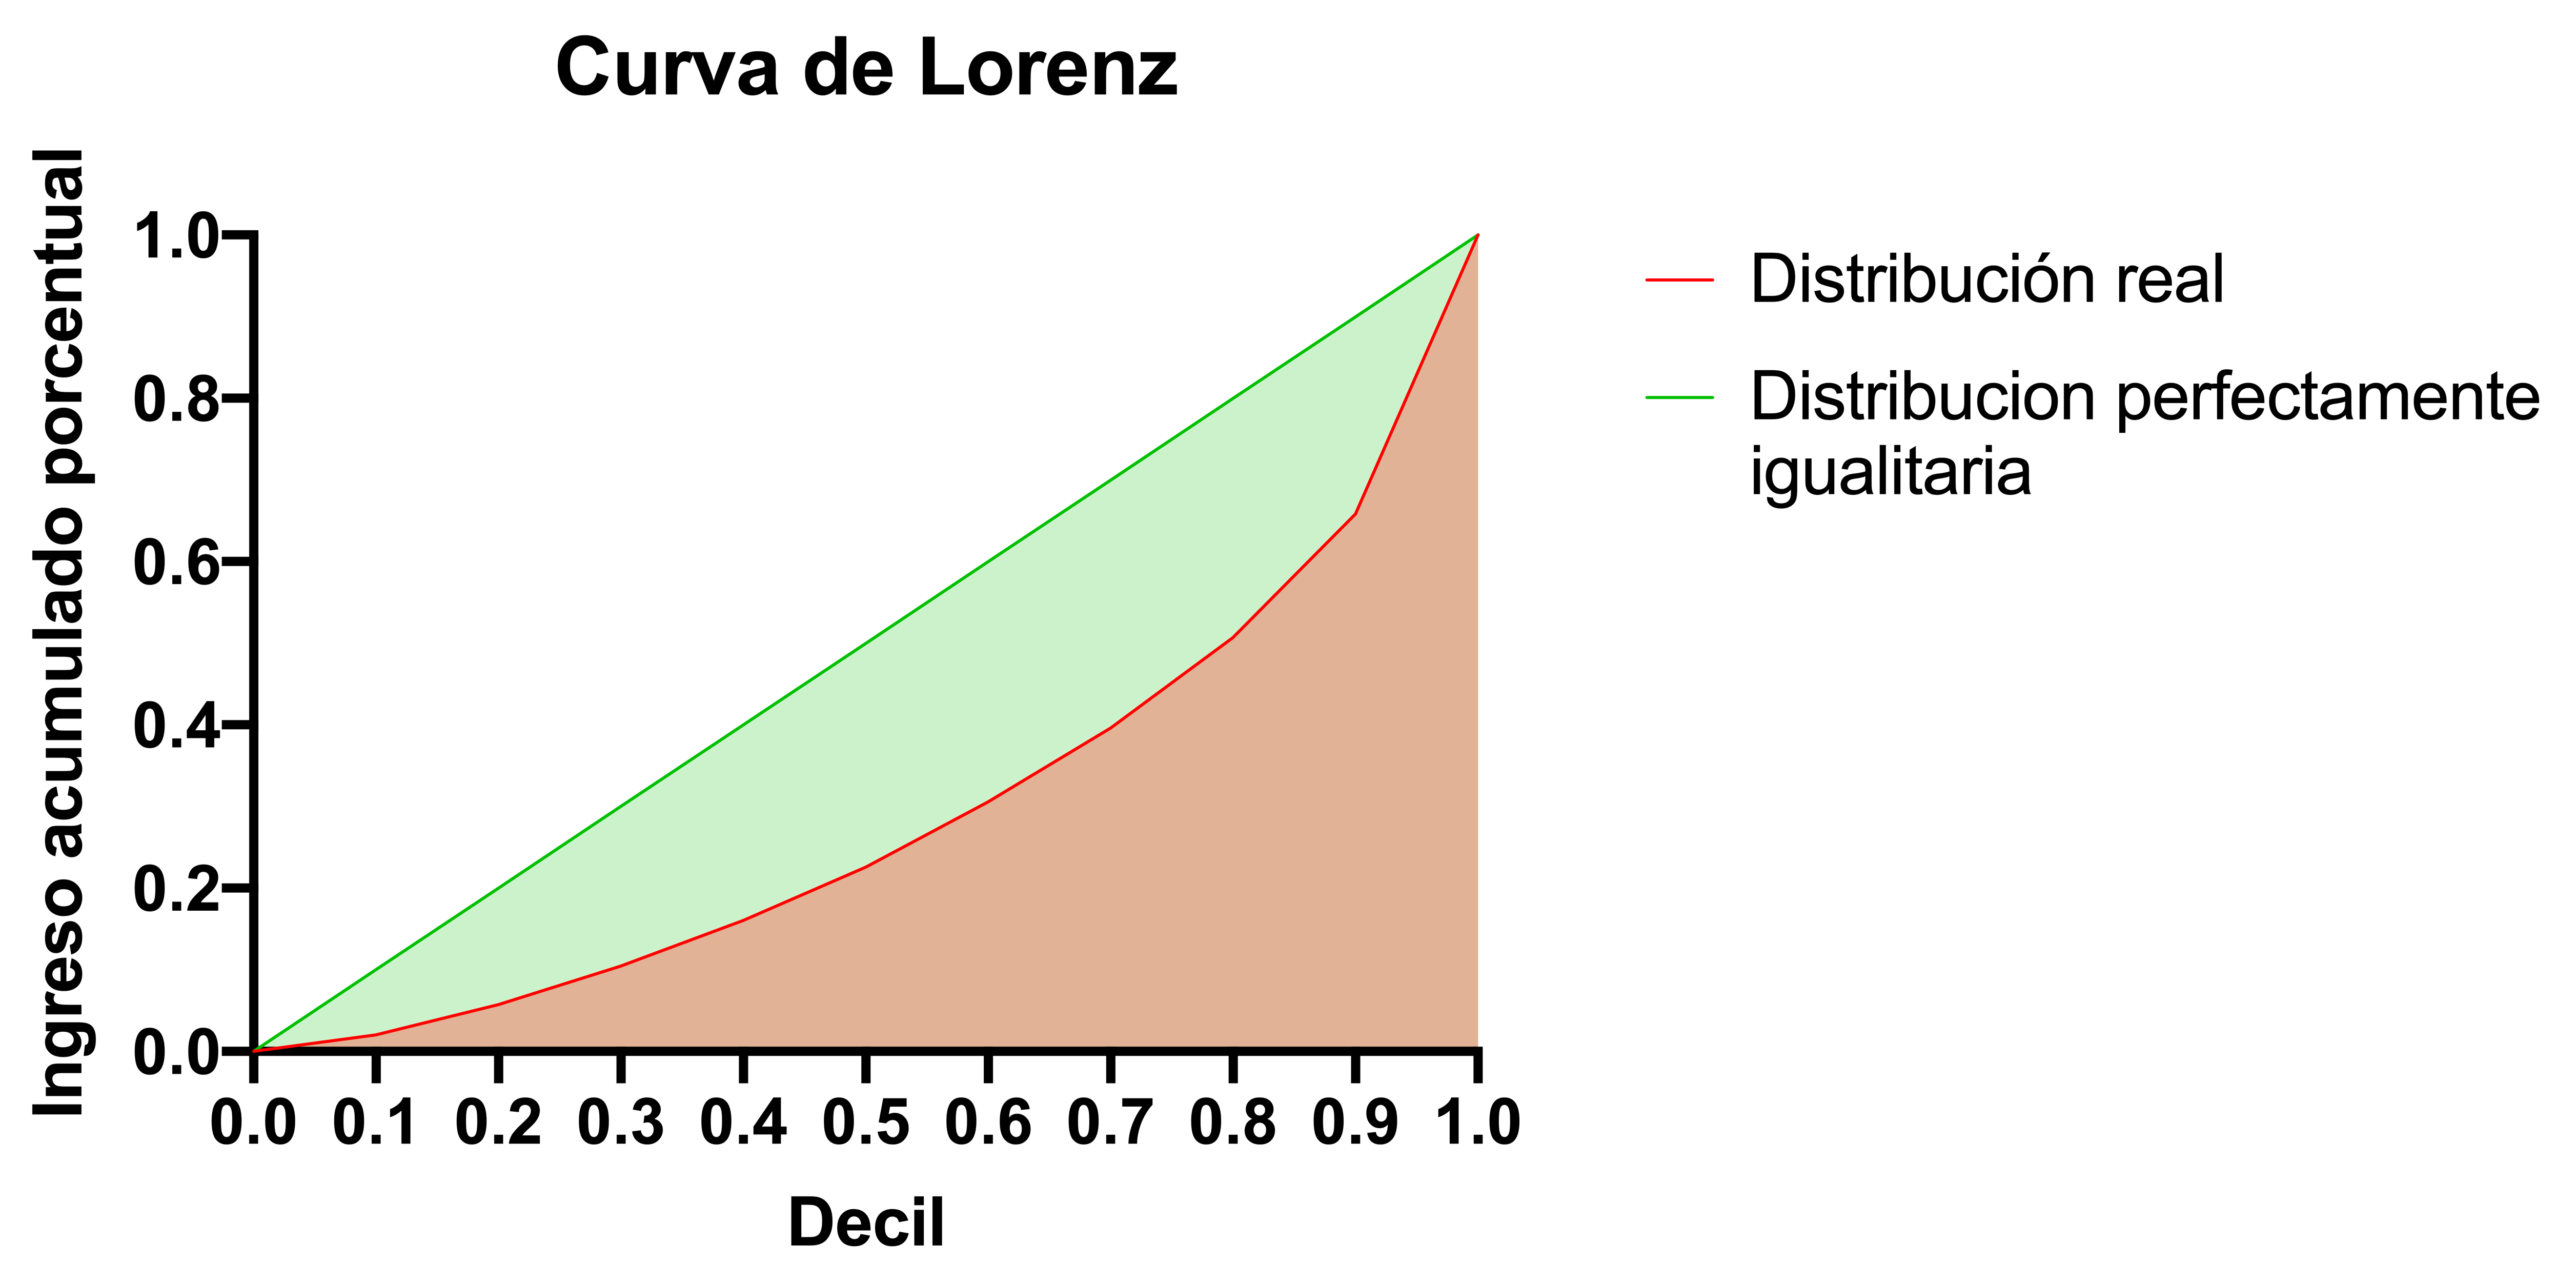
\includegraphics[width=0.84\textwidth]{Modulo_4/Curva_Lorenz_Final.png}
    \caption{Curva de Lorenz correspondiente a Chile, Casen 2017}
    \label{fig:lorenz_casen_2017}
\end{figure}

La figura \ref{fig:lorenz_casen_2017} muestra la curva de Lorenz correspondiente a Chile según la encuesta Casen 2017. En esta se puede observar en el eje vertical el \textit{Ingreso acumulado porcentual} y en el eje horizontal el \textit{Decil correspondiente} donde $0.1$ corresponde al decil 1, y así sucesivamente. \hfill \break


El índice de Gini se puede calcular a partir de las áreas bajo la curva del gráfico. Dividiendo el área entre la curva de la DPI y la distribución real, y sobre el área total. 
\[G = \frac{A_{DPI} - A_{DR}}{A_{total}}\]


En el caso de la figura \ref{fig:lorenz_casen_2017}, correspondería a dividir el área verde sobre la suma de las áreas verde y naranja. 
\newpage
\section{Criterios de asignación}

\econ{https://www.core-econ.org/the-economy/book/es/text/05.html}{5}

\subsection{Criterios de asignación}
Se entiende una asignación como el resultado de un determinado proceso económico.

\subsection{Eficiencia de Pareto}
Sean $A$ y $B$ asignaciones, la eficiencia de pareto establece que:
\hfill \break
\hfill \break
\textit{La asignación $A$ prevalece sobre la asignación $B$, si al menos una de las partes estaría mejor con $A$ que con $B$, y nadie estaría peor. En este caso $A$ domina a $B$ en términos de Pareto.}
\hfill \break


Una asignación que no está dominada en términos de Pareto se denomina \textbf{Pareto-eficiente.}


Este criterio es lo que en matemáticas se conoce como un orden parcial. Es decir, permite ordenar algunas asignaciones, pero no todas (esto sería un orden completo).

\subsubsection{Comentarios sobre la eficiencia de Pareto}
El criterio de la eficiencia de Pareto es uno de los conceptos más relevantes en economía. 


Dado un problema determinado, pueden existir muchas asignaciones que son pareto-eficientes. Pero sin un criterio adicional, no podemos decir cual de ellas es preferible.


Que una asignación sea eficiente de Pareto, no significa que estemos de acuerdo con ella. De hecho, si se le entregara todo el ingreso a una persona en la sociedad y dejamos a todo el resto sin nada, esa asignación es Pareto-Eficiente, pero probablemente no estemos de acuerdo en que sea una buena asignación económica.


Además, en muchas ocasiones, existe más de una asignación eficiente en términos de Pareto.

\subsection{Asignaciones}
Existen distintos casos posibles, y según este la manera de calcular asignación óptima varía.


\href{https://www.youtube.com/watch?v=jWcbHlTCPnQ}{Video EOL}
\begin{enumerate}[label=\Roman*.]
    \item \textbf{La persona genera el bien por si misma} \textit{(\href{https://youtu.be/jWcbHlTCPnQ?t=64}{Min 1:04})}, aquí $TMS = TMT$ es la condición de asignación óptima. 
    
    \item \textbf{Coerción} \textit{(\href{https://youtu.be/jWcbHlTCPnQ?t=181}{Min 3:01})}: alguien obliga a la persona a trabajar y se queda con los excedentes luego de darle lo mínimo que necesita la persona para subsistir (esclavitud). Existe una \textit{restricción de supervivencia biológica (RSB)}.
    
    El coerzor escogerá el punto donde la distancia entre la frontera del conjunto factible y la curva de RSB sea mayor.\\
    
    $TMB = TMT$ es la asignación óptima. (TMB es la tasa relacionada con RSB)
    
    \item \textbf{Propiedad privada} \textit{(\href{https://youtu.be/jWcbHlTCPnQ?t=333}{Min 5:33})}: La otra persona tiene todo el poder de negociación pero la primera persona solo trabajará si obtiene ganancias. \\
    
    Alguien externo (e.g. Estado o familia) ofrece una producción de sobrevivencia.\\
    
    Existe una curva de indiferencia de la primera persona. Se busca maximizar la distancia entre esa curva y la frontera factible.\\
    
    $TMT = TMS$ es la condición de optimalidad.
    
    \item \textbf{Negociación colectiva} \textit{(\href{https://youtu.be/jWcbHlTCPnQ?t=510}{Min 8:30})}: La primera persona busca parte del excedente.\\
    
    Una \hyperlink{institucion}{institución} externa (e.g. Estado) establece una curva de indiferencia nueva que ha de cumplirse, no necesariamente es Pareto-eficiente.\\
    
    A la persona se le puede ofrecer una nueva curva de indiferencia que le deje con igual igual utilidad (y que cumpla lo propuesto por el Estado) o que deje a ambas partes mejor.\\
    
    $TMT = TMS$ es la condición de optimalidad.
\end{enumerate}

\subsection{Desigualdad (criterios)}
Existen distintos tipos de medida a la hora de medir desigualdad, entre estas están

\begin{itemize}
    \item \textbf{Desigualdad absoluta}: es la resta de ingresos. Posee un problema que es que posee unidades dimensionales de ingreso lo cual hace difícil comparar entre lugares que no poseen las mismas unidades monetarias. Además aumenta cuando el país crece, aunque ambos ingresos crezcan a la misma \textit{tasa}. $\quad DA = Y_R - Y_P$
    
    \item \textbf{Desigualdad relativa}: es la división entre los ingresos. Es adimensional y no aumenta trivialmente cuando el país crece. $\quad DR = Y_R/Y_P$
\end{itemize}

Por esto es preferible hacer uso de la desigualdad relativa.

\subsubsection{Razones o \textit{ratios} de desigualdad}
Es la medida más sencilla de desigualdad, es la razón entre los ingresos de los sectores más ricos y pobres de la sociedad.

\begin{itemize}
    \item Razones entre quintiles
    \item Razones entre deciles
\end{itemize}

\subsubsection{Razón o índice de Palma}
Es un refinamiento de los \textit{ratios}, este índice considera que hay 3 grupos en la sociedad
\begin{enumerate}[label=\arabic*)]
    \item Los ricos (decil 10)
    \item Clase media (Decil 5 a 9)
    \item Los pobres (Decil 1 a 4)
\end{enumerate}

Se sustenta con la observación empírica: la clase media tiende a capturar la mitad del ingreso. 

\[\text{Razón de palma} = \frac{D_{10}}{D_1+D_2+D_3+D_4}\]

\subsubsection{Coeficiente o índice de Gini}
Es la medida más usada de desigualdad, representa que tanto se aleja una distribución real de una distribución totalmente igualitaria. Su valor varía entre 0 y 1, siendo mínima la desigualdad en 0 y máxima en 1. Posee dos formas:

\begin{enumerate}[label=\roman*.]
    \item \textbf{Forma general}: promedio de las diferencias de ingreso entre todos los individuos en una economía. Se calcula como \newline
    \[G = \frac{\sum_i\sum_j\abs{y_i-y_j}}{2\sum_{ij}y_i}\]
    
    \item \textbf{Forma de Sen}: suma ponderada de ingresos. (más usada)
    \newline
    \[G = \frac{2}{n}\frac{\sum_i^n i y_i}{\sum_i^n y_i} - \frac{n+1}{n}\]
\end{enumerate}


Donde $y_i$ son los ingresos correspondientes a $i$, e $i$ pueden ser deciles, quintiles, personas, etc. de las que hay una cantidad $n$.
\\

La interpretación más usual del coeficiente de Gini es a partir de la curva de Lorenz.
\subsubsection{Curva de Lorenz}
Muestra los ingresos acumulados desde los individuos más pobres a los más ricos de la sociedad. Comparándolos con la curva correspondiente a una distribución perfectamente igualitaria (DPI).

\begin{figure}[H]
    \centering
    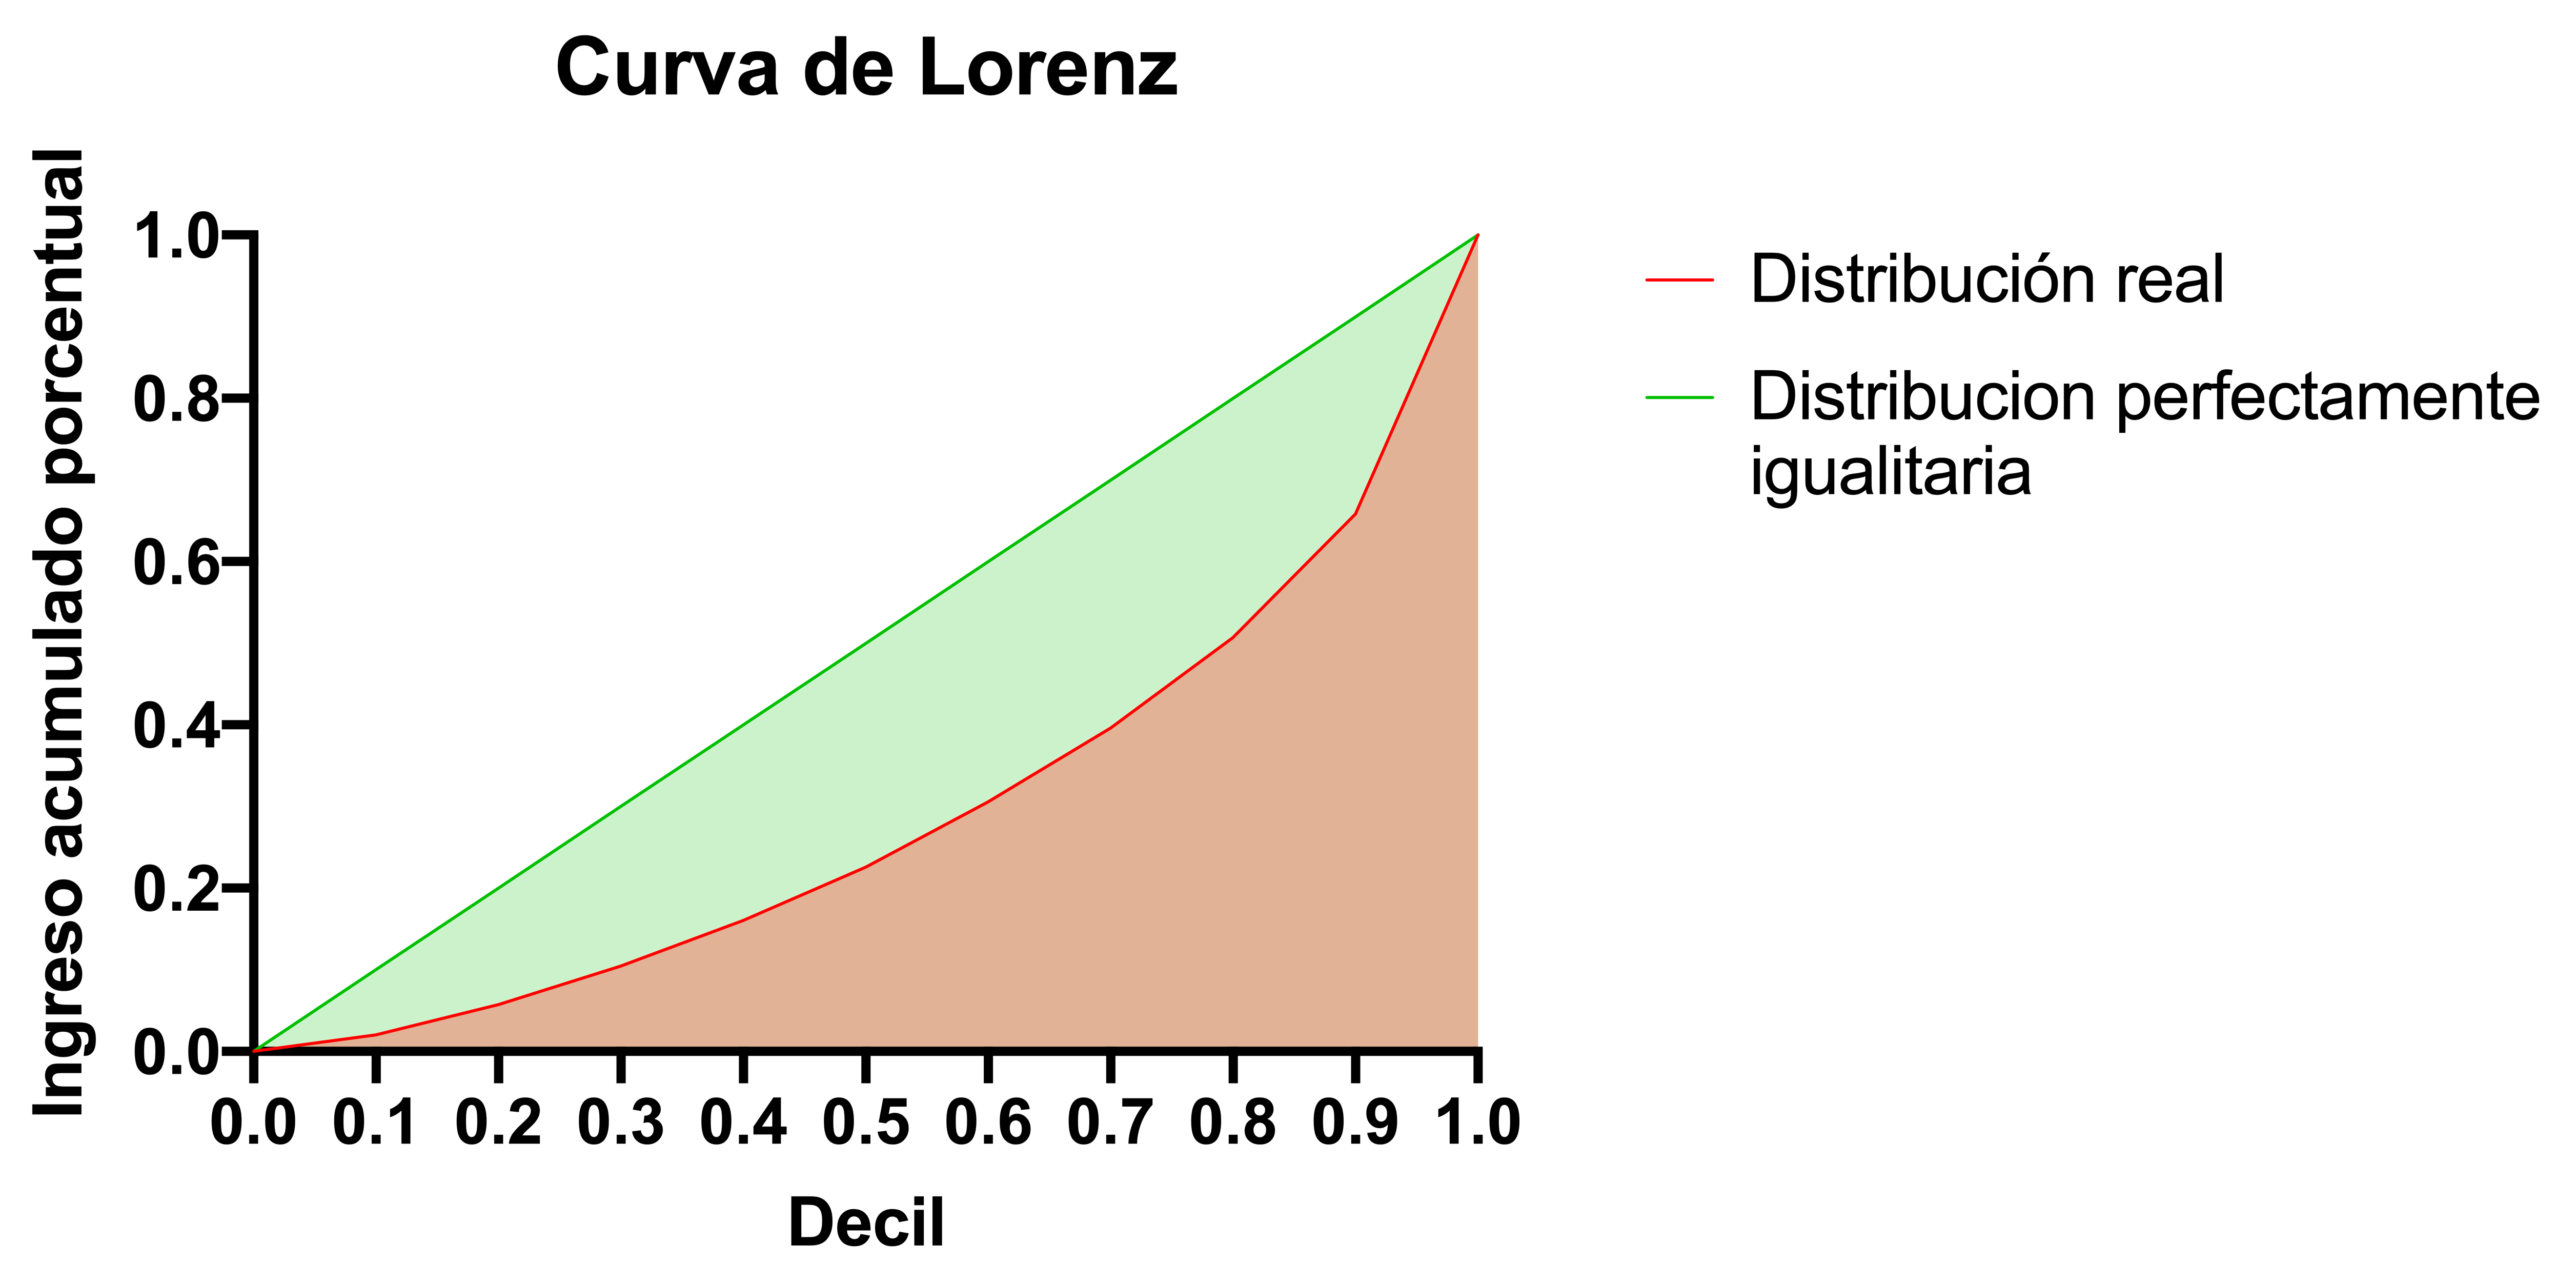
\includegraphics[width=0.84\textwidth]{Modulo_4/Curva_Lorenz_Final.png}
    \caption{Curva de Lorenz correspondiente a Chile, Casen 2017}
    \label{fig:lorenz_casen_2017}
\end{figure}

La figura \ref{fig:lorenz_casen_2017} muestra la curva de Lorenz correspondiente a Chile según la encuesta Casen 2017. En esta se puede observar en el eje vertical el \textit{Ingreso acumulado porcentual} y en el eje horizontal el \textit{Decil correspondiente} donde $0.1$ corresponde al decil 1, y así sucesivamente. \hfill \break


El índice de Gini se puede calcular a partir de las áreas bajo la curva del gráfico. Dividiendo el área entre la curva de la DPI y la distribución real, y sobre el área total. 
\[G = \frac{A_{DPI} - A_{DR}}{A_{total}}\]


En el caso de la figura \ref{fig:lorenz_casen_2017}, correspondería a dividir el área verde sobre la suma de las áreas verde y naranja. 
\newpage

\titleformat{\section}
  {\Large\bfseries}{\thesection.}{1px}{}

\section{Videos EOL}

\subsection*{Módulo 0: Introducción a la economía}

\begin{itemize}
    \item[-] \href{https://www.youtube.com/watch?v=Bk_XdL-Yq2E}{Bienestar, crecimiento y desigualdad.}
    
    \item[-] \href{https://www.youtube.com/watch?v=QhNrHly3Kd8}{Especialización del trabajo, intercambio y mercados.}

\end{itemize}

\subsection*{Módulo 1: Uso de modelos matemáticos en la economía}

\begin{itemize}
    \item[-] \href{https://www.youtube.com/watch?v=PhbLaTLzIAk}{Función de producción y Trampa de Malthus.}
    
    \item[-] \href{https://www.youtube.com/watch?v=DXGO7kK1uXI}{Tecnología, costos e innovación.}
    
    \item[-] \href{https://www.youtube.com/watch?v=-bYKV0pErEA}{Tutorial regresión lineal.}
    
\end{itemize}

\subsection*{Módulo 2: Escasez}

\begin{itemize}
    \item[-] \href{https://www.youtube.com/watch?v=P29Zd1-FGxE}{Motivación y función producción.}
    
    \item[-] \href{https://www.youtube.com/watch?v=R7monXl_M4E}{Preferencias y tomas de decisión.}
    
    \item[-] \href{https://www.youtube.com/watch?v=J-MyCczFGZc}{Salario y Efectos.} (Efecto ingreso y sustitución)
    
    \item[-] \href{https://www.youtube.com/watch?v=6gd_bGovblk}{Explicando Diferencias y Conclusión.}
    
\end{itemize}

\subsection*{Módulo 3: Teoría de Juegos}

\begin{itemize}
    \item[-] \href{https://www.youtube.com/watch?v=2B01O0VaJg4}{Presentación del módulo.}
    
    \item[-] \href{https://www.youtube.com/watch?v=Dh2AqD6h9nI}{Motivación y definiciones básicas.}
    
    \item[-] \href{https://www.youtube.com/watch?v=fKQ_5sbB9pI}{Estrategias dominadas.}
    
    \item[-] \href{https://youtu.be/S5mZmz6Q3PE}{Equilibrio de Nash.}
    
\end{itemize}

\subsection*{Módulo 4: Criterios de asignación}

\begin{itemize}
    \item[-] \href{https://youtu.be/VmjpxTykH5s}{Evaluación de Asignaciones.}
    
    \item[-] \href{https://youtu.be/jWcbHlTCPnQ}{Determinación de asignaciones.}
    
    \item[-] \href{https://youtu.be/PnxKqsnTKOM}{Desigualdad.}
    
\end{itemize}

\subsection*{Módulo 5: Monopolios}

\begin{itemize}
    \item[-] \href{https://youtu.be/WADyP3bQrH4}{Motivación}
    
    \item[-] \href{https://youtu.be/5jgzGaegmcY}{El problema del monopolio.}
    
    \item[-] \href{https://youtu.be/aORZTXIdOHw}{Relación entre la demanda y el margen monopólico.}
    
    \item[-] \href{https://youtu.be/VMXx_u8HF00}{Ineficiencia, monopolios naturales y regulación.}
    
\end{itemize}

\subsection*{Módulo 6: Discriminación de precios y tarificación}

\begin{itemize}
    \item[-] \href{https://www.youtube.com/watch?v=NR6JSmtmvkA}{Segmentos de mercado y monopolista}
    
    \item[-] \href{https://www.youtube.com/watch?v=pkvyhRhybI4}{Segmentación y discriminación de precios}
    
    \item[-] \href{https://www.youtube.com/watch?v=HlnLgL_2_jg}{Discriminación por volumen}
    
    \item[-] \href{https://www.youtube.com/watch?v=xHRb9aZVXUA}{Captura de excedentes}
    
\end{itemize}

\subsection*{Módulo 7: Oligopolio}

\begin{itemize}
    \item[-] \href{https://www.youtube.com/watch?v=dAHkFh1iNvk}{Motivación y definición}
    
    \item[-] \href{https://www.youtube.com/watch?v=lz5_zY4xf_Y}{Modelo de Cournot}
    
    \item[-] \href{https://www.youtube.com/watch?v=MC0dFTZrMXk}{Eficiencia, concentración y estructura de mercado}
    
    \item[-] \href{https://www.youtube.com/watch?v=aPzrelUix5w}{Política de competencia} 
    
\end{itemize}

\newcommand{\ytem}[2]{\item[-] \href{#1}{#2}}

\subsection*{Modulo 8: Mercados competitivos y firmas tomadoras de precios}

\begin{itemize}
    \ytem{https://www.youtube.com/watch?v=waAob5x6Cu4}{Introducción}
    
    \ytem{https://www.youtube.com/watch?v=WUn693uV38A}{Oferta, demanda y equilibrio de mercado}
    
    \ytem{https://www.youtube.com/watch?v=9vpN6H6RV2g}{Cambios en la oferta y demanda}
    
    \ytem{https://www.youtube.com/watch?v=ACTfimO_lXA}{Impuestos y subsidios}
    
\end{itemize}

\subsection*{Modulo 9: Fallas de Mercado y Externalidades}

\begin{itemize}
    \ytem{https://www.youtube.com/watch?v=OjlhIaO1YxQ}{Presentación del módulo}
    
    \ytem{https://www.youtube.com/watch?v=WJwVzEfAYmI}{Eficiencia y Externalidades}
    
    \ytem{https://www.youtube.com/watch?v=n8oAss-o59k}{Correción de Fallas}
    
    \ytem{https://www.youtube.com/watch?v=iccZWCPPwhA}{Otras fuentes de ineficiencia}
    
\end{itemize}

\newpage
\section{Glosario de términos}

\textit{Glosario de términos del CORE ECON (Puede buscar con ctrl+f o cmd+f)} \href{https://www.core-econ.org/the-economy/book/es/text/50-02-glossary.html#glossary-econom}{\textbf{IR}}

\begin{itemize}
    
    \item \hypertarget{trade-off}{\textbf{Trade Off}}: decisión tomada en una situación conflictiva en la cual se debe perder, reducir cierta cualidad a cambio de otra cualidad. En economía se lo suele traducir como 'intercambio', destacando entonces que se pierde un beneficio y se gana otro. \textit{[Fuente: Wikipedia]}
    
    \item \hypertarget{equilibrio}{\textbf{Equilibrio}}: Resultado autosostenible de un modelo. En este caso, algo de interés no cambia, a menos que se introduzca una fuerza externa que altere la descripción de la situación que proporciona el modelo. \textit{[Fuente: CORE]}
    
    \item \hypertarget{subsistencia}{\textbf{Nivel de subsistencia}}: Nivel de vida (medido en términos del consumo o el ingreso) al que la población no crece ni decrece. \textit{[Fuente: CORE]}
    
    \item \hypertarget{rendimiento-decreciente}{\textbf{Rendimiento decreciente}}: Situación en la cual el uso de una unidad adicional de un insumo de producción resulta en un menor incremento en el producto, respecto al incremento anterior. \textit{También se conoce como: rendimientos marginales decrecientes de la producción.} \fuente{CORE}
    
    \item \hypertarget{utilidad}{\textbf{Utilidad}}: Indicador numérico de valor que uno asigna a un resultado, de modo que se escojan resultados de mayor valor por encima de otros de menor valor cuando ambos sean factibles. \fuente{CORE}
    
    \item \hypertarget{frontera-factible}{\textbf{Frontera factible}}: Curva de puntos que define la máxima cantidad factible de un bien para una cantidad dada de otro. \fuente{CORE}
    
    \item \hypertarget{poder}{\textbf{Poder}}: capacidad de hacer y obtener las cosas que queremos, en contraposición con las intenciones de los demás.
    
    \item \hypertarget{instituciones}{\textbf{Instituciones}}: son reglas escritas y no escritas que rigen qué hacen las personas cuando interactúan en un proyecto común, y la distribución de los productos resultantes de su esfuerzo conjunto.
    
    \item \hypertarget{ex-ante}{\textbf{Ex-ante}}: significa "antes del suceso". Ex-ante se usa más comúnmente en el mundo comercial, donde los resultados de una acción concreta, o una serie de acciones, se prevén con antelación (o eso se pretende).
    
\end{itemize}

\newpage
\section{Misceláneo}

\subsection{Módulo 6}

\subsubsection{\cita{Mismo bien}}
\label{misc:mismo_precio}
¿Como se define un mismo bien?\\

Diferencias geográficas pueden causar diferencia de costes para un mismo producto, a causa de los costes de producción.\\


¿Si los bienes son distintos, habría discriminación?\\

Se podría discriminar sin que el bien sea exactamente el mismo (calidad del bien/servicio es distinta).\\


Se toma como un \cita{mismo bien}, uno casi indistinguible de otro.

\newpage




\section{Ejemplos}

\subsection{Costo de oportunidad}

\fuente{CORE}

Imagine que se les ha pedido a un contador y a un economista que informen sobre el costo de ir a un concierto \textit{A}, en un teatro, con una entrada cuyo costo asciende a 25 dólares. En un parque cercano hay un concierto \textit{B}, que es gratuito, pero que se celebra al mismo tiempo.
\\

\textbf{contador}:
el costo del concierto \textit{A} es el costo entendido como «lo que sale de su bolsillo»: usted ha pagado 25 dólares por una entrada, por lo tanto, el costo es 25 dólares.
\\

\textbf{economista}
¿Pero a qué tiene que renunciar para ir al concierto \textit{A}? Usted ha dado 25 dólares, más el disfrute del concierto gratuito en el parque. Así que el costo del concierto para usted es el costo en términos de lo que sale de su bolsillo más el costo de oportunidad.
Suponga que lo máximo que hubiera estado dispuesto a pagar para asistir al concierto gratuito en el parque (si no fuera gratuito) fueran 15 dólares. Entonces su beneficio, si es que eligiera su siguiente mejor alternativa al concierto \textit{A}, sería de 15 dólares de disfrute en el parque. Este es el costo de oportunidad de ir al concierto \textit{A}.
\\

Así que el costo económico (costo de bolsillo de una acción + costo de oportunidad) total del concierto \textit{A} es 25 dólares + 15 dólares = 40 dólares. Si anticipa que el goce que experimentará por ir al concierto \textit{A} es 50 dólares, dejará pasar el concierto \textit{B} y comprará la entrada para el teatro, porque 50 dólares es más que 40 dólares. Por otro lado, si anticipa que el goce que experimentará en el concierto \textit{A} es 35 dólares, entonces el costo económico de 40 dólares indica que no escogerá ir al teatro. En términos simples: dado que tiene que pagar 25 dólares por la entrada, optará por el concierto \textit{B} y se guardará los 25 dólares para gastarlos en otras cosas y disfrutar así de un beneficio valorado en 15 dólares resultante de ir al concierto gratuito en el parque.

\subsection{Discriminación primer grado}
\label{ejem:disc_1er_grado}
\begin{itemize}
    \item $1^{\text{er}}$ caso: el médico de un pueblo pequeño
    \item El monopolista fija precios diferentes para cada consumidor y para cada consulta comprada por cada uno de ellos
    \item Información: el monopolista (médico) puede identificar a cada consumidor.
    \item Arbitraje o fuga: no es posible
    \item Precios: diferentes para cada consumidor y unidad
\end{itemize}

\subsection{Discriminación de segundo grado}
\label{ejem:disc_2do_grado}
\begin{itemize}
    \item \textit{A} valora en \$3 la primera unidad, en \$2 la segunda, y \$1 la tercera.
    \item \textit{B}valora en \$4 la primera unidad, en \$3 la segunda, y en \$2 la tercera.
    \item Curva de Demanda: $(\$4, 1)$, $(\$3,3)$, $(\$2,5)$, $(\$1,6)$
    \item Mejor precio ($CMg = 0$)=\$2. Se venden 5 unidades a \$10.
    \item Si se tiene una unidad \$3, dos unidades \$4.8, tres unidades a \$6.5\\
    \textit{A} compra dos unidades, \textit{B} compra 3 unidades (Se auto-segmentan). Se venden 5 unidades en \$11.3
\end{itemize}

\newpage

\end{document}
